\pdfoutput=1
%\documentclass[lettersize,journal]{IEEEtran}
%\documentclass[onecolumn,12pt]{IEEEtran}
\documentclass[acmsmall,nonacm]{acmart}

% FOR ARXIV
%\documentclass[manuscript,nonacm]{acmart}

% FOR Submission
%\documentclass[manuscript,review]{acmart}

% Final
% \documentclass[acmsmall]{acmart}

\usepackage{amsmath,amsfonts}

\acmJournal{CSUR}

\usepackage{dsbda-style}
\usepackage{hyperref}

\usepackage{booktabs}
\usepackage{multirow}
\usepackage{multicol}
\usepackage{xspace}
\usepackage{threeparttable}
\usepackage{longtable}

\newcommand{\mlp}{WideMLP\xspace}

\newcommand{\mytextsubscript}[1]{{\color{black}\textsubscript{#1}}}
\newcommand{\myheader}{}

\newcommand{\GenLM}{generative language model\xspace} 
\newcommand{\GenLMs}{generative language models\xspace}

\newcommand{\SLM}{SLM\xspace}
\newcommand{\SLMs}{SLMs\xspace}
\newcommand{\LLM}{LLM\xspace}
\newcommand{\LLMs}{LLMs\xspace}

\let\mycite\cite
\newcommand\myflag[0]{our experiment}
%\let\mytablefontsize\small
\let\mytablefontsize\footnotesize

% \usepackage{cite}

\begin{document}

\title{Are We Really Making Much Progress in Text Classification? A Comparative Review}

%\author{Lukas Galke, Ansgar Scherp, Andor Diera, Bao Xin Lin, \\
%Bhakti Khera, Tim Meuser, Tushar~Singhal, and Fabian~Karl
%\thanks{L. Galke is with the University of Southern Denmark}
%\thanks{A. Scherp, A. Diera, B. Lin, B. Khera, T. Meuser, and F. Karl are with the University of Ulm, Germany}
%}

\author{Lukas Galke}
\orcid{0000-0001-6124-1092}
\affiliation{\institution{University of Southern Denmark}
\city{Odense}
\country{Denmark}}
\email{galke@imada.sdu.dk}

\author{Ansgar Scherp}
\orcid{0000-0002-2653-9245}
\affiliation{\institution{University of Ulm} \country{Germany}}
\email{ansgar.scherp@uni-ulm.de}

\author{Andor Diera}
\orcid{0009-0001-3959-493X}
\affiliation{\institution{University of Ulm} \country{Germany}}
\email{andor.diera@uni-ulm.de}

\author{Fabian Karl}
\orcid{0009-0008-0079-5604}
\affiliation{\institution{University of Ulm} \country{Germany}}
\email{fabian.karl@uni-ulm.de}

\author{Bao Xin Lin}
\affiliation{\institution{University of Ulm} \country{Germany}}
\email{bao.lin@uni-ulm.de}

\author{Bhakti Khera}
\affiliation{\institution{University of Ulm} \country{Germany}}
\email{bhakti.khera@uni-ulm.de}

\author{Tim Meuser}
\affiliation{\institution{University of Ulm} \country{Germany}}
\email{tim.meuser@uni-ulm.de}

\author{Tushar Singhal}
\affiliation{\institution{University of Ulm} \country{Germany}}
\email{tushar.singhal@uni-ulm.de}

\begin{CCSXML}
<ccs2012>
   <concept>
       <concept_id>10010147.10010257.10010258.10010259.10010263</concept_id>
       <concept_desc>Computing methodologies~Supervised learning by classification</concept_desc>
       <concept_significance>500</concept_significance>
       </concept>
   <concept>
       <concept_id>10002944.10011122.10002945</concept_id>
       <concept_desc>General and reference~Surveys and overviews</concept_desc>
       <concept_significance>500</concept_significance>
       </concept>
   <concept>
       <concept_id>10002951.10003317.10003347.10003356<concept_id>
       <concept_desc>Information systems~Clustering and classification</concept_desc>
       <concept_significance>300</concept_significance>
       </concept>
   <concept>
       <concept_id>10010147.10010257.10010293.10010294</concept_id>
       <concept_desc>Computing methodologies~Neural networks</concept_desc>
       <concept_significance>500</concept_significance>
       </concept>
 </ccs2012>
\end{CCSXML}

\ccsdesc[500]{Computing methodologies~Supervised learning by classification}
\ccsdesc[500]{Computing methodologies~Neural networks}
\ccsdesc[500]{General and reference~Surveys and overviews}
\ccsdesc[300]{Information systems~Clustering and classification}

\renewcommand{\shortauthors}{Galke et al.}

\begin{abstract}

We analyze various methods for single-label and multi-label text classification across well-known datasets, categorizing them into bag-of-words, sequence-based, graph-based, and hierarchical approaches. 
Despite the surge in methods like graph-based models, encoder-only pre-trained language models, notably BERT, remain state-of-the-art. 
However, recent findings suggest simpler models like logistic regression and trigram-based SVMs outperform newer techniques. 
While decoder-only generative language models show promise in learning with limited data, they lag behind encoder-only models in performance. 
We emphasize the superiority of discriminative language models like BERT over generative models for supervised tasks. 
Additionally, we highlight the literature's lack of robustness in method comparisons, particularly concerning basic hyperparameter optimizations like learning rate in fine-tuning encoder-only language models.

\noindent \textbf{Data availability}: The source code is available at \url{https://github.com/drndr/multilabel-text-clf}. All datasets used for our experiments are publicly available except the NYT dataset.

\end{abstract}

\maketitle
\clearpage
\tableofcontents
\clearpage

%\begin{IEEEkeywords}
%Data mining, text mining, text classification, neural networks, machine learning
%\end{IEEEkeywords}

\section{Introduction}

\subsection{Motivation and Background}

Text classification is the task of assigning a categorical label or multiple of such labels to a given text unit~\cite{DBLP:journals/csur/Sebastiani02,DBLP:journals/tkde/MoreoES20}. 
It is a central task in natural language processing, with numerous practical applications, such as classifying scholarly documents, social media posts, news articles, or email spam.
Unsurprisingly, until now, text classification has been a very active research field, with new methods appearing every week, as reflected by recent surveys~\cite{
DBLP:journals/tkde/HuLZHNL24,
fieldsSurveyTextClassification2024,
electronics13071199,
DBLP:journals/tist/LiPLXYSYH22,
DBLP:journals/csur/MinaeeKCNCG21,
DBLP:journals/corr/abs-2107-03158,
raihan2021-survey,
DBLP:journals/wias/ZhouGLVTBBK20, 
DBLP:journals/information/KowsariMHMBB19,
DBLP:journals/air/Kadhim19}. 

Besides the rapid pace of research in text classification, conceptually new approaches have also emerged that are not yet sufficiently covered in existing surveys. Those include the use of graph neural networks (GNNs) to process text, which attracts increasing attention from researchers, and the rise of large language models (LLMs), which are often (naively) assumed to be the state-of-the-art in all-natural language processing tasks. 
Although there are surveys with good coverage of new methods, \eg focusing on LLMs~\cite{DBLP:journals/tkde/HuLZHNL24} or GNNs~\cite{gnns-for-nlp-survey}, those then lack a quantitative comparison. 
Other surveys perform a quantitative comparison but focus on single-label classification and use their own splits instead of the established splits per dataset~\cite{DBLP:journals/eswa/ReusensSTSVBB24}.
This survey covers both of these new families alongside classical approaches and provides a quantitative comparison across multi-class (or single-label), multi-label, and hierarchical text classification.

Many new methods for text classification are based on graph neural networks (GNNs)~\cite{book:hamilton:grl}.
Common to these GNN-based approaches is that they first generate a synthetic graph from the corpus that contains text-augmented vertices and edges with information on word and document co-occurrences, \eg~\cite{DBLP:conf/aaai/YaoM019,texting_acl2020}. 
Second, the GNN is trained on this graph to carry out the text classification task.
In hierarchical text classification, where classes are organized along a thematic hierarchical thesaurus~\cite{DBLP:journals/csur/Sebastiani02}, GNNs are often used to encode the label hierarchy, \eg~\cite{hbgl,DBLP:conf/acl/WangWH0W22}.

Another group of text classification methods is based on language models, which can be organized in encoder-only, encoder-decoder, and decoder-only models~\cite{yang2023harnessing}.\footnote{Disclaimer:
We are well aware of the vivid discussions and evolving organization of language models, \eg on social media like LeCun's post \url{https://twitter.com/ylecun/status/1651762787373428736} that encoder-only models of course also have a decoder, but ``just not an auto-regressive decoder'', etc.    
We follow the key distinction between language models as discussed by LeCun and surveys such as Yang et al.~\cite{yang2023harnessing}.
We focus on the central aspect of distinguishing language models for classification tasks, \ie between fine-tuned discriminative models versus generative large language models as this distinction, central to our observations in the survey, as it also corresponds to whether task-specific fine-tuning is employed.
}
Encoder-only pre-trained language models such as BERT~\cite{DBLP:conf/naacl/DevlinCLT19} took big strides in many natural language processing tasks including categorical text classification~\cite{galke2023really,galkescherp-acl2022}. 
The encoder-only transformer language models were followed by encoder-decoder variants T5~\cite{T5} and decoder-only generative large language models (\LLMs) such as the GPT models-~\cite{DBLP:journals/corr/abs-2303-08774,DBLP:conf/nips/BrownMRSKDNSSAA20}.
Decoder-only transformer language models focus on text generation with remarkable in-context learning abilities.
This makes them strong zero-shot and few-shot models~\cite{carp,DBLP:conf/iclr/PatelLRCRC23,wei2022finetuned,DBLP:conf/nips/BrownMRSKDNSSAA20}, 
yet whether in-context learning LLMs are superior to fine-tuned small language models is highly questionable~\cite{DBLP:conf/acl/QoribMN24,
bucher2024finetunedsmallllmsstill,
lepagnol2024smalllanguagemodelsgood,
liu2024llmembedrethinkinglightweightllms,
edwards2024language,
li2023label}.

Decoder-only language models are usually much larger than masked language models~\cite{DBLP:conf/nips/BrownMRSKDNSSAA20}, which is because the causal language model objective architecture (left-to-right prediction) allows for easier scaling through diagonal masking of the attention matrices -- enabling the model to get an error signal for each token in a batch.
Thus, we increasingly find the distinction between \SLMs (small language models) and \LLMs, \eg~\cite{DBLP:conf/aaai/Hu0CSLW024,DBLP:journals/corr/abs-2402.12819,DBLP:journals/corr/abs-2402-16844}, which is based on a (kind of arbitrarily) chosen parameter count.
We argue that a key distinction between \SLMs and \LLMs, particularly for classification tasks, lies in the pre-training objective.
The encoder-only and encoder-decoder \SLMs (\eg BERT and T5) are based on masked language modeling (with subsequent fine-tuning of a discriminative classifier in BERT and its variants) while the decoder-only \LLMs (\eg GPTs) are pre-trained using the causal language modeling objective.
This side-effect of pre-training objectives is not by coincidence but rather an effect of the causal language model objective providing a training signal for each token, whereas the masked language model objective only provides a training signal for each \emph{masked} token.

Another side effect of scale is that \SLMs are usually fine-tuned for a specific downstream task. Although task-specific fine-tuning is also possible with \LLMs through techniques like Low-Rank Adaptation~\cite{lora}, it is more prohibitive due to the higher number of parameters with common model, such that most approaches leveraging \LLMs rely on more general instruction fine-tuning~\cite{ouyangTrainingLanguageModels2022} followed by in-context learning with few examples and dedicated prompting schemes~\cite{carp}.

\subsection{What is the Problem? Why is our Study Needed?}

Encoder-only language models like BERT have led to major improvements to the state of the art on many NLP tasks, including categorical text classification~\cite{galke2023really,galkescherp-acl2022}.
Our question here is whether the numerous newly proposed methods provide substantial improvements over encoder-only language models. 
We pinpoint this question to three aspects analyzed in this paper, namely the apparent ineffectiveness of using synthetic graphs, the importance of task-specific fine-tuning, even in the era of  \LLMs, and the general challenges of fairly assessing new methods and baselines.

\begin{itemize}
    \item  \textit{Synthetic Graphs}
The use of GNNs has been specialized to the task of text classification by synthetic graphs induced from the text corpus, \eg TextGCN~\cite{DBLP:conf/aaai/YaoM019}.
However, those synthetic graphs may not provide information beyond what a neural network can already directly extract from the text~\cite{galkescherp-acl2022}.

\item \textit{Large Language Models}
The literature suggests that generative \LLMs do not generally improve over encoder-only \SLM for text classification tasks~\cite{DBLP:journals/corr/abs-2402-07470-pushing-the-limit,
carp,
yuan2023revisiting,
li2023chatgpt,
yu2023open}.
This comes despite the strong advantages of generative \LLMs in their sheer size of parameters as well as improvements based on techniques like prompt engineering~\cite{carp,chain-of-thought}, 
instruction fine-tuning~\cite{wei2022finetuned}, and prompt-tuning~\cite{liu-etal-2022-p,lester-etal-2021-power}.

\item \textit{Comparability of Methods}
A general challenge when assessing the performance of methods is the comparability of the results.
Besides properly reporting the used datasets, splits, preprocessing, etc. an important question is if baselines are properly optimized~\cite{DBLP:conf/recsys/DacremaCJ19,leech2024questionablepracticesmachinelearning}. 
It is especially challenging to properly compare methods for text classification when so many new papers appear using GNNs and language models.
\end{itemize}

\subsection{Methodology}

We extensively review the literature in the field of modern and classical machine learning methods for single-label and multi-label text classification.
Based on the literature search, we derive the families of methods for text classification. 

\begin{itemize}
\item Methods based on Bag of Words (BoW) using, \eg a support vector machine or a multi-layer perceptron~\cite{galkescherp-acl2022}.

\item Methods that consider text as a sequence of tokens such as the encoder-only BERT~\cite{DBLP:conf/naacl/DevlinCLT19} or the decoder-only GPT~\cite{DBLP:conf/nips/BrownMRSKDNSSAA20}, 

\item Graph-based methods that employ graph neural networks on synthetic graphs like TextGCN~\cite{DBLP:conf/aaai/YaoM019} and hierarchy-based text classification methods like HGCLR~\cite{DBLP:conf/acl/WangWH0W22}.
\end{itemize}

We determine established single-label and multi-label benchmark datasets, which we consider in our comparison, and identify the top-performing methods.
We carefully probe the validity of the results for each method and paper found in the literature.
We check, among others, the train-test split used (whether they deviate from established benchmark splits), 
the number of classes considered, 
the hyperparameter values (are they provided and comparable, 
whether the baselines are optimized, 
the metrics applied, 
and if there is any unusual preprocessing of the datasets that may have influenced the results.  

We aggregate all results found in the literature.
We identified gaps in the use of methods and datasets, \ie when certain combinations of models and datasets could not be found.
Where needed, we run own experiments to fill gaps.
Overall, we achieve a systematic comparison of the different text classification methods among the different families of methods.

\subsection{Key Results}
The family of fine-tuned transformer language models defines the state of the art for single-label and multi-label text classification tasks.
Despite recent advances in \LLMs, the best-performing models for text classification are still \SLMs BERT and its variants RoBERTa~\cite{liu_roberta:_2019} and DeBERTa~\cite{he_deberta_2021}.
Despite their sheer amount of parameters and larger pretraining, methods based on in-context learning with \LLMs do not generally outperform fine-tuned \SLMs in text classification.
Even when pushing the limit of using such \GenLMs by applying tricks such as advanced prompting techniques~\cite{carp} or using ensembles~\cite{DBLP:journals/corr/abs-2402-07470-pushing-the-limit}, the performance does not, or only marginally on individual datasets, outperform those of encoder-only \SLMs. 
For example, it requires an ensemble of Llama \LLMs to reach or slightly outperform an encoder-only \SLM on two benchmark datasets~\cite{DBLP:journals/corr/abs-2402-07470-pushing-the-limit}.
We attribute these observations to two main factors.
First, task-specific fine-tuning is still an important distinctive criterion.
The encoder-only models like BERT are pre-trained with the masked language modeling objective and fine-tuned with a classifier head for specific datasets on the text classification task.
Second, the left-to-right attention mask is suboptimal for text classification tasks.
Therefore, fine-tuned models with unrestricted attention are effective text classifiers and should be preferred over purely generative models for text classification tasks.
This again relates well to the distinction between generative and discriminative approaches~\cite{DBLP:conf/sigir/Nallapati04} -- the former aiming to learn the full joint distribution $p(x,y)$, which we interpret here as in-context learning, and the latter focusing on the decision boundary directly, \ie $p(y|x)$, which we interpret here as task-specific fine-tuning.

For the GNN-based methods, despite the huge number of methods developed in recent years, the idea of exploiting a synthetically induced graph to improve text classification has not lived up to its promise.
Many graph-based methods such as \cite{DBLP:conf/aaai/YaoM019,DBLP:conf/aaai/LiuYZWL20,DBLP:conf/wsdm/RageshSIBL21} are not only outperformed by simply applying BERT but already fall below simple baselines such as a logistic regression or a simple classifier such as a multi-layer perception on a bag-of-words representation~\cite{galkescherp-acl2022,DBLP:conf/wsdm/RageshSIBL21}.
Such baseline models already extract relevant information for text classification from the raw text~\cite{DBLP:journals/csur/Sebastiani02}.
Adding a synthetically generated graph from the corpus does not provide additional information that a neural network can exploit~\cite{galkescherp-acl2022}.

A worrying observation is the lack of strong baselines and/or not properly tuning them appropriately.
Like Dacrema, Cremonesi, and Jannach~\cite{DBLP:conf/recsys/DacremaCJ19} observed for neural recommender systems that ``works can be outperformed at least on some datasets by conceptually and computationally simpler algorithms'', the reason is also that baselines are not properly optimized~\cite{DBLP:conf/recsys/ShehzadJ23} (``everyone's a winner'').
Classical machine learning methods such as support vector machines, logistic regression, and multi-layer perceptrons are largely ignored in papers published in the last years, despite showing consistently strong results across various datasets~\cite{galke2023really,galkescherp-acl2022,DBLP:conf/wsdm/RageshSIBL21}.
There are cases where even the baseline's most basic hyperparameter, the learning rate (or fine-tuning learning rate, in the case of BERT models) is not properly considered.
We show this in the example of BERT and its variants, which makes these models perform considerably worse compared to what they can achieve.
The literature shows a quite high discrepancy in BERT's performance on benchmark datasets, up to a $13$ points difference in accuracy, which can be attributed to the choice of the fine-tuning learning rate.

Following studies in other areas of machine learning, we conclude that strong baselines must be used and their hyperparameters properly optimized as it is an important means to argue about \textit{true} scientific advancement~\cite{DBLP:conf/acl/HenaoLCSSWWMZ18,DBLP:conf/recsys/DacremaCJ19}, and also their usefulness in practical settings.

\subsection{Remainder}

The remainder of this article is organized as follows: 
Below, we introduce our survey methodology.
We survey the literature along the families of methods for text classification, beginning with BoW-based models in \Secref{sec:bow}, sequence-based methods in \Secref{sec:sequence}, and concluding with graph-based methods in \Secref{sec:graph}.
The experimental apparatus, including the considered datasets, and the procedure for running our own experiments to fill gaps in the literature is described in \Secref{sec:apparatus}.
The results of our quantitative comparison are presented in \Secref{sec:results}.
Subsequently, we discuss limitations in \Secref{sec:limitations}, findings in \Secref{sec:findings}, and promising future directions in \Secref{sec:future}, before concluding.

\section{Methodology}\label{sec:sota}

This survey covers single-label text classification, multi-label text classification, and hierarchical text classification -- covering published methods up to January 2025.
We do not consider \emph{extreme} multi-label classification, where the focus is dealing with very large label space, which requires a different set of specialized techniques~\cite{xml0,xml4,xml3,xml2} and different metrics (ranking metrics rather than classification metrics), whose comparison we leave for future work. 

In a first step, we have collected and analyzed recent surveys on single-label and multi-label text classification and searched for research papers that include comparison studies~\cite{
wang2023graph,
duarte2023review,
buguenoConnectingDotsWhat2023,
DBLP:journals/tist/LiPLXYSYH22,
DBLP:journals/csur/MinaeeKCNCG21,
DBLP:journals/pr/TarekegnGM21,
DBLP:journals/corr/abs-2107-03158,
raihan2021-survey,
DBLP:journals/wias/ZhouGLVTBBK20,
DBLP:conf/esann/QaraeiKB20,
DBLP:journals/corr/abs-2011-11197,
DBLP:journals/information/KowsariMHMBB19,
DBLP:journals/air/Kadhim19,
galkescherp-acl2022,
DBLP:conf/jcdl/MaiGS18,
DBLP:conf/kcap/GalkeMSBS17,
DBLP:conf/sigir/ZhangWYWZ16}.
These cover the range from classical machine learning models to deep classification models.
Second, we have screened for literature in key NLP and artificial intelligence venues.
Finally, we have complemented our search by checking results and papers on \url{https://paperswithcode.com/task/text-classification} (for single-label) and \url{https://paperswithcode.com/task/multi-label-text-classification} (for multi-label).

Based on this input, we have determined the families of methods and benchmark datasets used (see Table~\ref{tab:datasets}).
This categorization is mainly based on the method signature, distinguishing whether methods operate on BoW, sequence, or graph-structured input~\cite{galkescherp-acl2022}. 
We extend the categorization by further distinguishing between two types of graph-based methods: 
First, approaches that employ a graph structure derived from a corpus of text documents, which we call synthetic text-graph approaches. 
Second, hierarchy-based methods that are using a graph model to encode the hierarchical structure among classes. 
We further add the subcategories of large language models and attention-free language models to the family of sequence-based models. 
\Figref{fig:one} shows an overview of the categorization.

We focus our analysis on methods that show strong performance and include them in our study.
We have verified that the same train-test split is used for all methods.
We check whether modified versions of the datasets have been used (\eg fewer classes) to avoid bias and mistakenly give advantages.

We do not consider papers that do not allow for a fair comparison with the state of the art.
Reasons include that they 
\begin{itemize}
\item used different or non-standard benchmark datasets only like \cite{
petridis2024textclassificationneuralnetworks,
peng2025text,
petridis2024textclassificationneuralnetworks,
DBLP:journals/nca/JiaJDZLXC23-mhgat,
10748883-boing-aviation-paper,
LMTCSG-10705790,
AGBESI2024e38515,
10.1007/978-3-031-72350-6_20,
DBLP:journals/corr/abs-2408-15650,
Wei_Sun_2024,
DBLP:conf/kdd/Yu00S24,
DBLP:conf/sigir/DaiYCX24, 
DBLP:journals/corr/abs-2403-03293, 
10.1016/j.datak.2024.102306,
DBLP:journals/access/ThaminkaewLV24,
DBLP:journals/tkde/HuLZHNL24,
DBLP:conf/coling/LyKCK24,
JAMSHIDI2024102306,
DBLP:journals/corr/abs-2401-01667-MLP-Compass,
thaminkaew2024ieeeaccess,
li2023chatgpt,yu2023open,yuan2023revisiting,
zhu2023,
chae_davidson_2023,
zhang2023pretraining,
Yang-ClimateChangeClassifiert-2023,
DBLP:journals/apin/TanRW23,
bgnn-xml,
DBLP:conf/ijcnn/TranSZPB22,
LiuEtAl2022-LongText,
DBLP:conf/aiia/BreazzanoC021a,
DBLP:journals/corr/abs-2206-07253,
DBLP:journals/corr/abs-2112-11389,
chalkidis-etal-2020-empirical,
DBLP:conf/eacl/SchwenkBCL17,gururangan-etal-2019-variational},

\item modified the datasets to use a different number of classes as done in \cite{DBLP:conf/coling/ZhouQZXBX16,DBLP:conf/aaai/LaiXLZ15,MTAPparlakNovelFeatureClassbased2023},

\item employed different train-test splits like
\cite{
donabauer2024tokenlevelgraphsshorttext,
DBLP:journals/eswa/ReusensSTSVBB24,
edwards2024language,
StylianouEtAl2023,
DBLP:journals/corr/abs-2211-02563,
DBLP:conf/ijcnn/SunHCYSM22,
raihan2021-survey,
DBLP:conf/icaart/PalSS20,
moreo2020,
canutoThoroughEvaluationDistanceBased2018}, 

\item train-test splits are not reported~\cite{moreo2020,sf-cnn-iasc.2023.027429,YuanEtAl-MSVM-kNN-2008},

\item used fewer training examples~\cite{
DBLP:conf/acl/LiangZ0Z24,
DBLP:conf/aaai/LiuZ0ZWMCYZ24,
Xie2024DataLT,
zhu2023,
duarte2023review,
DBLP:journals/corr/abs-2301-10481,
DBLP:conf/emnlp/ZhengWYD22,
DBLP:conf/ijcnn/SunHCYSM22,DBLP:conf/emnlp/WangWYD21}, 
or

\item used different evaluation measures~\cite{tan2022,DBLP:conf/emnlp/HuangGKOO21}.

\end{itemize}

The rationales for why certain changes are made were not always clear in the literature.
However, it reflects a general problem of comparability in machine learning research~\cite{leech2024questionablepracticesmachinelearning}.

Below, we describe the family of BoW methods in detail in \Secref{sec:bow}, 
sequence-based methods in \Secref{sec:sequence}, and graph-based methods in \Secref{sec:graph}. 

\begin{figure*}
    \centering
    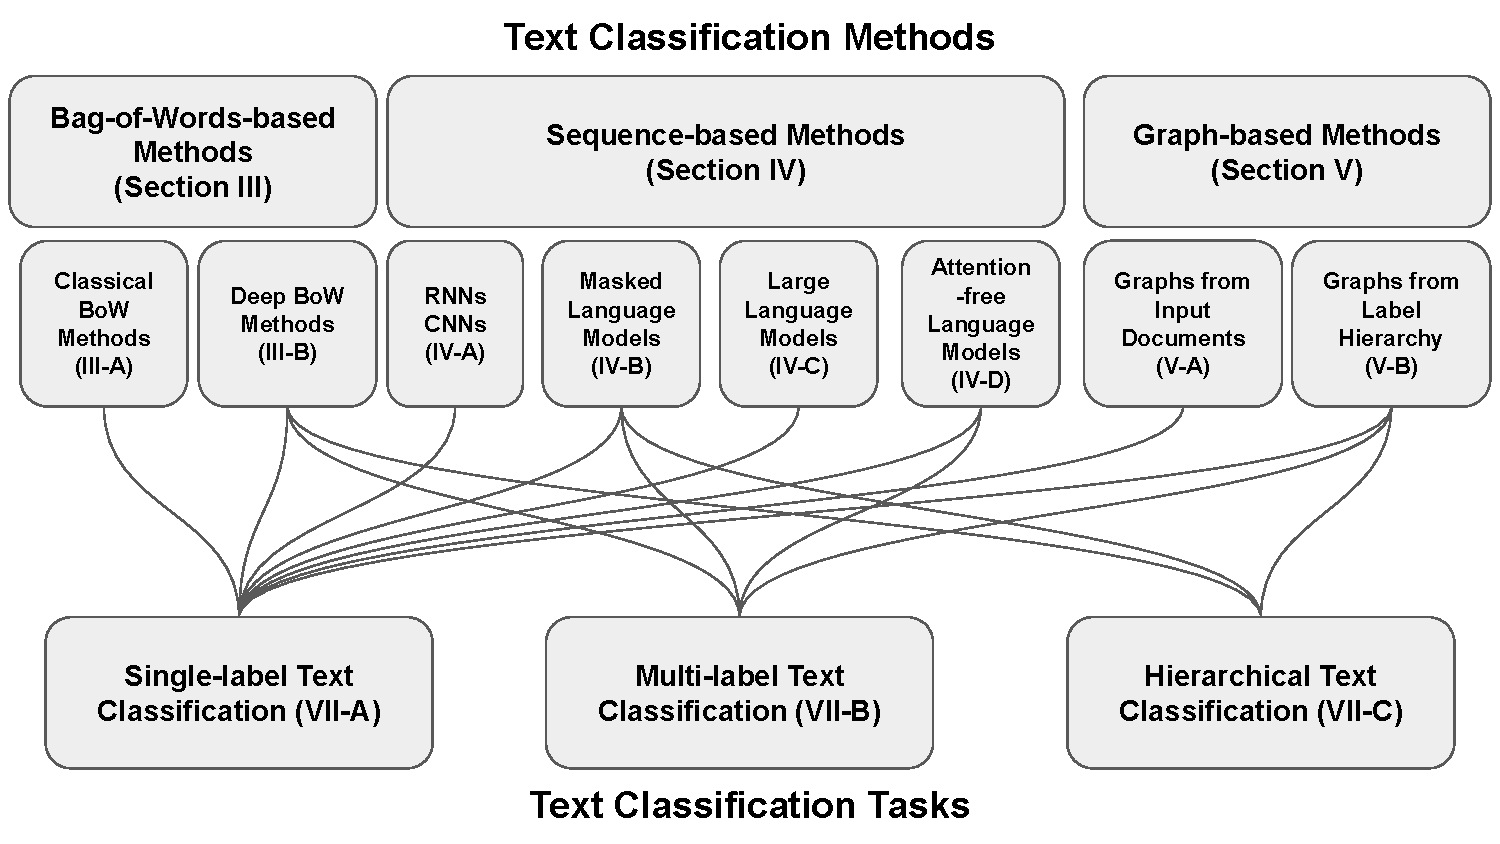
\includegraphics[width=0.8\textwidth]{TextClfSurvey-Figure1}
    \caption{Categorization of text classification methods in families (top) and tasks (bottom). 
    We draw a line if at least one of the combinations of method and task is covered in our quantitative comparison.}
    \label{fig:one}

\end{figure*}

\section{BoW-based Methods}\label{sec:bow}
Under pure BoW-based (Bag of Words) text classification, we denote approaches that operate only on a multiset of words (or tokens) from the input document. 
Given paired training examples $(\vx,y) \in \train$, each consisting of a vector that holds the frequency of words in its components $\vx \in \sR^{n_\mathrm{vocab}}$, which is commonly referred to as a bag (multiset) of words, and a class label $y \in \sY$. 
The goal is to learn a generalizable function $\hat\vy = f_\theta^{(\mathrm{BoW})}(\vx)$ with parameters $\theta$ such that $\operatorname{arg\,max}(\hat\vy)$ is the true label $y$ for input $\vx$.
For multi-label classification, the BoW-based model considers multiple class labels. 
Instead of using $\operatorname{arg\,max}(\hat\vy)$ to decide on a label, a binary sigmoid output is commonly used per label and, along with a threshold $\lambda$ that determines whether the corresponding class will be assigned. 
The multi-label model is trained with a binary cross-entropy loss instead of a categorical cross-entropy.
As output, the multi-label classifier can produce between $0$ to $|\sY|$ many labels~\cite{DBLP:journals/csur/Sebastiani02}, \ie it is possible that no label is predicted.

\subsection{Classical BoW Methods}

Classical machine learning methods that operate on a BoW-based input are extensively discussed in surveys and comparison studies~\cite{
DBLP:conf/wsdm/RageshSIBL21,
DBLP:journals/information/KowsariMHMBB19,
DBLP:journals/air/Kadhim19,
DBLP:conf/kcap/GalkeMSBS17}.
These studies show that the best-performing classical models are Support Vector Machines (SVM) and logistic regression (LR).
Especially, the strong performance of logistic regression is astonishing.
For instance, Ragesh~\etal\cite{DBLP:conf/wsdm/RageshSIBL21} have shown that logistic regression outperforms the advanced graph-based TextGCN~\cite{DBLP:conf/aaai/YaoM019} method. 

\subsection{Deep BoW Methods}

With more advanced BoW methods, Galke~\etal\cite{DBLP:conf/kcap/GalkeMSBS17} have found that an MLP on a bag-of-words representation of the text outperforms many graph-based approaches.
Earlier approaches are mainly based on pre-trained word embeddings~\cite{DBLP:conf/nips/MikolovSCCD13,DBLP:conf/emnlp/PenningtonSM14}.
For instance, Iyyer~\etal\cite{DBLP:conf/acl/IyyerMBD15} proposed Deep Averaging Networks (DAN), a combination of word embeddings and deep feedforward networks.
DAN is an MLP with one to six hidden layers, non-linear activation, dropout, and AdaGrad as an optimization method.
The results suggest that pre-trained embeddings such as GloVe~\cite{DBLP:conf/emnlp/PenningtonSM14} would be preferable over randomly initialized neural bag-of-words~\cite{DBLP:conf/acl/KalchbrennerGB14}.
In fastText~\cite{DBLP:journals/tacl/BojanowskiGJM17,DBLP:conf/eacl/GraveMJB17}, a linear layer is used on top of pre-trained embeddings for classification.
Furthermore, Henao~\etal\cite{DBLP:conf/acl/HenaoLCSSWWMZ18} explore different pooling variants for the input word embeddings and find that their Simple Word Embedding Models (SWEM) can rival approaches based on recurrent (RNN) and convolutional neural networks (CNN).
Note that approaches such as fastText and SWEM that apply a logistic regression on top of pre-trained word embeddings share a similar architecture as an MLP with one hidden layer. 
However, the standard training protocol involves pre-training the word embedding on large amounts of unlabeled text and then freezing the word embeddings while training the logistic regression~\cite{DBLP:conf/nips/MikolovSCCD13}.

\section{Sequence-based Methods}\label{sec:sequence}
As sequence-based methods, we consider recurrent and convolutional neural networks, \SLMs (\eg BERT), \LLMs (\eg GPT-3.5), and attention-free language models (e.g., gMLP). 
These approaches aim for \emph{contextualized} word representations, for which nearby words and word order are taken into account.
The model signature for sequence-based methods is
$\hat{y} = f_\theta^{(\mathrm{sequence})} ( \langle x_1, x_2, \ldots, x_k \rangle )$,
where $k$ is the (maximum) sequence length.

\subsection{Recurrent and Convolutional Neural Networks}

Before the era of pre-trained language models, recurrent neural networks (RNN) were a natural choice for any NLP task.
SGM is a model for multi-label classification based on a bidirectional LSTM with an attention mechanism~\cite{sgm}, which later has been extended to use T5 as a backbone language model~\cite{seq2tree}.
BLSTM-2DCNN~\cite{DBLP:conf/coling/ZhouQZXBX16} is a bidirectional LSTM with two-dimensional max pooling.
It has been applied to a subset of the 20ng dataset with four classes. 
Thus, the high score of $96.5$ reported for 4ng cannot be compared with papers applied to the full 20ng dataset, such as \cite{galkescherp-acl2022}.
Also Text\-RCNN~\cite{DBLP:conf/aaai/LaiXLZ15}, a model combining recurrence and convolution 
uses only the four major categories in the 20ng dataset. 
The results of Text\-RCNN are identical to BLSTM-2DCNN.
For the MR dataset, BLSTM-2DCNN provides no information on the specific split of the dataset.
RNN-Capsule~\cite{DBLP:conf/www/WangSH0Z18} is a sentiment analysis method reaching
an accuracy of $83.80$ on the MR dataset but with a different train-test split.
Lyu and Liu~\cite{DBLP:journals/corr/abs-2006-15795} combine a 2D-CNN with bidirectional RNN.
Another work applying a combination of a convolutional layer and an LSTM layer is by Wang~\etal\cite{DBLP:conf/ijcnn/WangLCCW19}. 
The authors experiment with five English and two Chinese datasets, which are not in the set of representative datasets we identified.
The authors report that their approach outperforms existing models like fastText on two of the five English datasets and both Chinese datasets. 

\subsection{Small Language Models}
The transformer~\cite{DBLP:conf/nips/VaswaniSPUJGKP17}, originally developed for machine translation, introduced a key-value self-attention mechanism, and had an immense impact on language modeling.
transformer-based language models are pre-trained with a self-supervised training objective on large text corpora and can be subsequently fine-tuned with a supervised objective on a specific task.
Generally, transformer-based language models can be categorized into encoder-only models, encoder-decoder models, and decoder-only models~\cite{yang2023harnessing}.
BERT and its follow-up approaches are encoder-only language models and are trained with the masked-language modeling objective~\cite{DBLP:conf/naacl/DevlinCLT19}.
Their main purpose is encoding the text and performing a classification or regression task with a dedicated module (\eg a linear output layer) on top of the encoder.
The output layer is trained from scratch (\ie from random initialization) during fine-tuning.

Encoder-decoder language models such as T5~\cite{T5} cast all downstream tasks, including classification, into a text-to-text framework with task-specific prompt prefixes. The rationale is that this practice enables multi-task fine-tuning with the aim of similar tasks improving each other.
Although these models generate text, they can also be used for classification tasks by interpreting generated tokens as class labels. 
In multi-label classification, text-to-text (= sequence-to-sequence) models have been used even before the era of large language models~\cite{namMaximizingSubsetAccuracy2017} to facilitate the prediction of multiple labels.

Popular follow-up works of BERT are
RoBERTa~\cite{liu_roberta:_2019}, DistilBERT~\cite{distilbert}, ALBERT~\cite{lan_albert_2020}, DeBERTa~\cite{he_deberta_2021}, and
ERNIE~2.0~\cite{sun_ernie_2019}.
RoBERTa improves the pre-training procedure of BERT and removes the next sentence prediction objective.
DeBERTaV3~\cite{DBLP:conf/iclr/HeGC23} is a modified DeBERTa with an ELECTRA-style pre-training~\cite{DBLP:conf/iclr/ClarkLLM20-electra}.
DistilBERT~\cite{distilbert} is a distilled version of BERT with 40\% reduced parameters and 60\% faster inference time that retains 97\% of BERT's performance on the GLUE benchmark.
ALBERT reduces the memory footprint and increases the training speed of BERT for improved scalability.
Like DistilBERT and ALBERT, TinyBERT~\cite{tinybert} and MobileBERT~\cite{sun2020mobilebert} are also size-reduced variants of BERT, but these two need the original BERT model for fine-tuning.
DeBERTa introduces a disentangled attention mechanism, \ie keeping word position and content embeddings separate, and an enhanced mask decoder, which introduces absolute position encodings to the final softmax.
ERNIE 2.0 employs a continual multi-task learning strategy. 
Whenever a new task is introduced, the previous model parameters are used for initialization, and the new task is added to the multi-task learning objective.
Finally, ModernBERT is a refurbished variant of the BERT model integrating various optimizations developed over the years and providing an input length of $8,192$ tokens~\cite{warner2024smarterbetterfasterlonger}.

Pre-trained language models have also found their way into hierarchical text classification.
For instance, HBGL~\cite{hbgl} uses BERT to represent the text and represent the hierarchically organized classes.
For the classes, HBGL first learns the label embeddings from the global hierarchy, \ie the taxonomy.
Specifically, the label embeddings are learned by employing a masked language modeling objective on sequences that correspond to paths in the label hierarchy.
Subsequently, it learns to predict the document labels one by one in the order of the local hierarchy, \ie level-wise from the root to the most specific label in the taxonomy.
By this, HBGL exploits the hierarchy of the labels as defined in the taxonomy and treats the label generation as a multi-label text classification task in a similar way as Nam et al.~ \cite{namMaximizingSubsetAccuracy2017} did with sequence-to-sequence models trained from scratch.
Thus, HBGL is essentially a \textit{hierarchy-aware} sequence-based transformer model. 
However, as described above, the key ingredient of HBGL is making use of the sequence-based model BERT.
HBGL \textit{does not use an external graph encoder} for representing the taxonomy.
In contrast, the graph-based methods (described in Section~\ref{sec:graph}) always use an \textit{explicit} graph encoder for representing the taxonomy, most commonly a graph neural network, independent of what other model is being used (\eg a CNN, BERT, or other).
Since HBGL's core is heavily based on BERT and does not have an explicit graph encoder, we consider it a sequence-based transformer method.

The encoder-decoder model Seq2Tree adopts T5 to perform hierarchical text classification~\cite{seq2tree}.
It uses a depth-first search approach to linearize the label hierarchy in order to encode it as a sequence in the model.
Finally, RADAr is a sequence-to-sequence model that uses RoBERTa as a text encoder and a custom two-layer Transformer-based decoder for hierarchical text classification~\cite{radar}.
In contrast to hierarchical text classification methods, see Section~\ref{sec:rw:hierarcy-based-methods}, RADAr does not operate on a given dataset taxonomy.
Beyond using ROBERTa as an encoder in RADAr, we also experimented with order transformer models, including BERT, XLNet, and DeBERTa. The results were generally very similar, with RoBERTa achieving the slightly highest scores overall.

Other approaches that use small language models for text classification include retrieval and data augmentation from an external knowledge base, such as Zhu~\etal~\cite{zhu2023}, who query ProBase to improve short text classification with BERT. For reasons of a fair comparison, we do not consider approaches that make use of an external knowledge base in our quantitative comparison.

\subsection{Large Language Models}

Decoder-only language models such as GPT-3~\cite{DBLP:conf/nips/BrownMRSKDNSSAA20} are trained with a left-to-right, \ie causal language modeling, objective. This makes decoder-only models most suitable for text generation. 
However, decoder-only models are very flexible and can also be used to carry out other downstream tasks, including text classification~\cite{DBLP:conf/nips/BrownMRSKDNSSAA20,radfordLanguageModelsAre}. 
This is done by specifying the task in natural language and providing a few examples in the prompt~\cite{DBLP:conf/nips/BrownMRSKDNSSAA20}. 
This practice, known as in-context learning, does not require updating the model. 
In-context learning has led to increased interest in the design of and working with prompts, such as Chain-of-Thought (CoT) prompting~\cite{weiChainofThoughtPromptingElicits2023} \emph{inter alia}.

The state-of-the-art prompting technique for text classification is Clue And Reasoning Prompting (CARP)~\cite{carp}, where the instructions consist of first finding relevant clues in the text input and then providing a classification result based on the clues along with an explanation. 

The recent work by Sun~\etal~\cite{carp} evaluates GPT-3.5+CoT on text classification and introduces a prompting strategy called Clue and Reasoning Prompting (CARP).
The authors evaluate GPT-3.5, GPT-3.5+CoT, and GPT-3.5+CARP with two different samplers for selecting the in-context examples.
The samplers are a uniform sampler and a RoBERTa model fine-tuned for the current downstream task.
Using RoBERTa representations of the training documents, the sampler employs a $k$NN search on the examples to sample more representative documents per class to be included in the prompt.
The best-performing CARP variant employs a 16-shot RoBERTa sampler with a majority vote over multiple runs of prompting GPT-3.5, which we denote as GPT-3.5+CARP+vote.

Specifically for text classification, prompt boosting has shown promising results
\cite{pmlr-v202-hou23b}, where differently prompted LLMs were ensembled with an adaptive boosting algorithm. 
However, the few-shot performance of large language models without any fine-tuning is still lower than fine-tuned small language models~\cite{edwards2024language}.
Beyond prompting techniques,
Zhang et al.~\cite{DBLP:journals/corr/abs-2402-07470-pushing-the-limit} have experimented with fine-tuning an ensemble of Llama-2~\cite{touvronLlamaOpenFoundation2023} models for text classification leading to competitive scores.
Li et al.~\cite{li2023label} do report promising results when fine-tuning a Llama-2 model~\cite{touvronLlamaOpenFoundation2023} without causal masking such that both left and right context can be considered during self-attention. 

In the end, it is currently unknown whether in-context learning with a large language model is sufficient for a given task or whether fine-tuning is needed. 

\subsection{Attention-free Language Models}
The self-attention mechanism has been very successful, but it has quadratic complexity in sequence length.
After transformer-based models have also entered the vision domain~\cite{visiontransformer}, Google researchers introduced methods that eliminate the costly self-attention mechanism in transformers and are purely based on MLP layers. 
The first of these attention-free models is MLP-Mixer \cite{tolstikhin2021mlp} developed for vision tasks. 
It divides the input image into a sequence of non-overlapping patches, then fed through blocks of MLPs consisting of channel-mixing and token-mixing layers.

Shortly after releasing the MLP-Mixer architecture, an MLP-based natural language processing model called gMLP~\cite{DBLP:journals/corr/abs-2105-08050} was released. 
The gMLP model replaces the attention layer in the basic blocks of a transformer with a spatial gating unit. 
Inside this layer, cross-token interactions are achieved by multiplying the hidden representation element-wise and projecting it linearly. 

While Liu et al.~\cite{DBLP:journals/corr/abs-2105-08050} found that it is possible to achieve similar performance as BERT by replacing self-attention with these gating units, gMLP was still outperformed by BERT on some tasks.
The authors hypothesized that self-attention could be advantageous depending on the tasks (\ie cross-sentence alignment).
Therefore, they attached a tiny attention unit (single-head with size $64$) to the gating units. 
This extension is called aMLP and substantially increases the model's performance.
While other attention-free language models have been proposed~\cite{pengRWKVReinventingRNNs2023a,guMambaLinearTimeSequence2023b}, none of them has been systematically evaluated for topical text classification.

\section{Graph-based Methods}\label{sec:graph}

Graphs can serve several purposes in text classification: One is to consider the input data as a graph (\ie the documents, their words), which we call synthetic text-graph approaches to distinguish them from graphs in which the structure has a natural interpretation (\eg citations graphs). Another purpose is considering an additional label hierarchy as input to the model~\cite{DBLP:journals/csur/Sebastiani02} (\ie classes organized in a hierarchy), which we call hierarchy-based methods.

\subsection{Synthetic Text-Graph Methods}

Using graphs induced from text has a long history in text classification. 
An early work is the term co-occurrence graph of the KeyGraph algorithm~\cite{DBLP:conf/adl/OhsawaBY98}.
The graph is split into segments, representing the key concepts in the document.
Co-occurrence graphs have also been used for automatic keyword extraction~\cite{Rose2010} and classification~\cite{DBLP:conf/emnlp/ZhangDXLZ21}.
Modern methods exploit this idea of a graph induced from the text.
The text corpus is first transformed into a graph, which is then fed as input into a graph neural network (GNN)~\cite{book:hamilton:grl}.

The synthetic text-graph approaches to text classification first set up a \emph{synthetic} graph based on the text corpus $\train$ such that an adjacency matrix is created from a document corpus $\hat\mA := \operatorname{make-graph}(\train)$.
The graph is composed of word nodes and document nodes, each receiving its own embedding (by setting $\mX =\mI$).
For example, in TextGCN, the graph is created from word-word edges (modeled by pointwise mutual information) and word-document edges (resembling word occurrence in the document).
Then, a parameterized function $f_\theta^{(\mathrm{graph})}(\mX, \hat\mA)$ is learned that uses the graph as input, where $\mX$ are the node features. 
Note that graph-based approaches such as TextGCN disregard word order, similar to the BoW-based models described above.

Among others, methods that follow this synthetic text-graph approach include
TextGCN~\cite{DBLP:conf/aaai/YaoM019},
TensorGCN~\cite{DBLP:conf/aaai/LiuYZWL20},
Hete\-GCN~\cite{DBLP:conf/wsdm/RageshSIBL21},
HyperGAT~\cite{DBLP:conf/emnlp/DingWLLL20}, 
HGAT~\cite{DBLP:journals/tois/YangHSJLN21},
DADGNN~\cite{DBLP:conf/aaai/LiuYZWL20}, 
STGCN~\cite{stgcn},
SHINE~\cite{DBLP:conf/emnlp/WangWYD21},
AGGNN~\cite{aggnn}.
While many of these methods are strictly transductive such as HeteGCN and TensorGCN, other methods are 
inductive~\cite{DBLP:conf/coling/HuangCC22,induct-gcn,texting_acl2020,DBLP:conf/emnlp/HuangMLZW19} or can be adapted to become inductive~\cite{DBLP:conf/wsdm/RageshSIBL21}.
Transductive models need access to the unlabeled test documents at training time. 
This requires computing the graph also on the documents of the test set and making this information available during training (but without the labels from the test set).
In contrast, inductive models can be applied to new data. 
Here, the graph induced from the text is computed only on the training set.

Transductive training has inherent drawbacks as the models cannot be applied to new documents.
For example, in TextGCN's original transductive formulation, the entire graph, including the unlabeled test set, must be available for training.
This may be prohibitive in practical applications as each batch of new documents would require retraining the model.
When TextGCN and other graph-based methods are adapted for inductive learning, where the test set is unseen, they achieve notably lower scores~\cite{DBLP:conf/wsdm/RageshSIBL21}. 
Note that all previously described bag-of-words and sequence-based models fall in the inductive category and can be applied to new documents.

We briefly discuss selected graph-based methods.
In TextGCN, the authors set up a graph with word and document nodes. Word--word edges are derived from pointwise mutual information (PMI) and word--document edges are derived from TF-IDF scores.
This synthetic graph is then fed into a graph convolutional network (\eg a GCN~\cite{DBLP:conf/iclr/KipfW17}) with the goal of classifying the document nodes.
HeteGCN combined ideas from Predictive Text Embedding~\cite{DBLP:conf/kdd/TangQM15} and TextGCN and splits the adjacency matrix into its word-document and word-word sub-matrices and fuse the different layers' representations when needed.
TensorGCN explores and combines multiple different ways of converting the text into a graph, such as a semantic graph created with an LSTM, a syntactic graph created by dependency parsing, and a sequential graph based on word co-occurrence. 
HyperGAT combines graph attention~\cite{velickovic2018graph} with the concept of hyperedges based on sequential structure and topic models~\cite{DBLP:journals/jmlr/BleiNJ03}.
AGGNN~\cite{aggnn} focuses on text pooling mechanism along with gated graph sequence neural networks~\cite{DBLP:journals/corr/LiTBZ15}.
DADGNN is a graph-based approach that uses attention diffusion and decoupling techniques for tackling the over-smoothing problem of the GNN and building deeper models. 
Lastly, STGCN tackles short text classification by building upon ideas from TextGCN and adding word-topic and document-topic edges from a topic model, similar to HyperGAT.
The authors also experimented with combining STGCN with a BiLSTM and a BERT model.
In their experiments, the combination STGCN+BERT+BiLSTM gave the best results, while pure STGCN fell behind pure BERT. MHGAT~\cite{mhgat} follows a different approach and captures word order by adding position-specific hyperedges to the graph to be processed by a graph attention network. These position edges are obtained through a sine/cosine transformation, following a similar strategy as in the Vaswani transformer's positional encoding ~\cite{DBLP:conf/nips/VaswaniSPUJGKP17}.

Particularly between 2022 and 2024, numerous new graph-based models have been published.
Many of them use BERT in conjunction \textit{with an explicit graph encoder}, usually a graph neural network, such as in BertGCN~\cite{DBLP:conf/acl/LinMSHKLW21}, CTGCN~\cite{ctgcn}, ILGCN~\cite{ilgcn}, TSW-GNN~\cite{tsw-gnn}, and ConTextING~\cite{DBLP:conf/coling/HuangCC22}.
They differ from the other GNN-based methods as the graph is not computed based on word co-occurrences but BERT's subword tokens.
Further graph-based methods are KGAT~\cite{DBLP:conf/nlpcc/WangWYZSJWZ22}, InducT-GCN~\cite{induct-gcn}, TextSSL~\cite{textssl2022}, GLTC~\cite{gltc2023}, and others.
A recent survey on GNNs for text classification was performed by Wang, Ding, and Han~\cite{wang2023graph}.
Moreover, Bugueno and de Melo~\cite{buguenoConnectingDotsWhat2023} compare different initial document representations including Word2vec~\cite{DBLP:conf/nips/MikolovSCCD13}, GloVe~\cite{DBLP:conf/emnlp/PenningtonSM14}, and frozen BERT embeddings and use them in conjunction with graph neural networks. 
They employ frozen and fine-tuned BERT models as baselines for the categorical text classification task. 
Their results show that---on most datasets---graph neural networks hardly compete with a fine-tuned BERT.

\subsection{Hierarchy-based Methods}
\label{sec:rw:hierarcy-based-methods}
Apart from the text-induced graphs used by the methods described above, also the classes of the dataset may be organized in a graph structure.
This is typically the case in hierarchical text classification, where each document should be annotated with a set of labels rather than a single class label~\cite{DBLP:journals/csur/Sebastiani02}. 
and the classes are organized along a taxonomy. 
The taxonomic hierarchy of labels is typically modeled as a tree or a directed acyclic graph~\cite{shen-etal-2021-taxoclass,hiagm,pengHierarchicalTaxonomyAwareAttentional2021}. 
The goal is then to predict multiple class labels which correspond to one or more nodes in the hierarchy.

Following the taxonomic hierarchy to the root, the classes become more general (broader), while going towards the leaves, the classes become more specific (narrower).
The documents are typically annotated with some specific classes in the taxonomy.
However, in hierarchical text classification, this taxonomy is often used to \emph{enrich} the gold standard~\cite{hiagm}. 
This means that all vertices along the entire path from the root to the assigned classes are added as ground truth.
The hierarchy-based text classifier HiAGM~\cite{hiagm} and its follow-up works, such as HGCLR~\cite{DBLP:conf/acl/WangWH0W22} and HBGL~\cite{hbgl}, rely on this enrichment.

The enrichment affects both the training and evaluation of hierarchy-aware methods.
After this enrichment, the dataset consists of a set of documents $\mX$. Each document is annotated with multiple labels, typically modeled as a label indicator matrix $\hat\mY$, and a hierarchy of classes $\mH$.
Then, the goal is to learn a function $\vx, \mH \mapsto \hat\vy$ that maps the current document $\vx$ to a set of enriched labels $\hat\vy$, while also taking into account the label hierarchy $\mH$. 
The hierarchy-based methods make use of an explicit graph encoder to represent the taxonomy and to exploit it in the model architecture to classify the text.

We briefly discuss the selected methods.
HiAGM is a hierarchical text classifier that models the hierarchy as a directed graph along with hierarchy-aware structure encoders~\cite{hiagm}.  
It comes in two variants: HiAGM-LA, which is a multi-label attention model that uses an inductive approach.  
HiAGM-TP is a text feature propagation model that uses a deductive approach to extract hierarchy-aware text features. It uses a GNN-based encoder to obtain a representation for each class and compare it with a Tree-LSTM representation of the text.  
In early 2021, several other hierarchical label-based attention models were published.  For example, HLAN \cite{dong2021explainable}, LA-HCN \cite{DBLP:journals/corr/abs-2009-10938}, RLHR~\cite{liu2021improving}, and the
weakly-supervised Taxo\-Class~\cite{shen-etal-2021-taxoclass}.
Further, hierarchy-based methods are
\cite{DBLP:journals/corr/abs-1812-11270,DBLP:journals/corr/abs-1902-09347,DBLP:journals/corr/abs-1909-00161}.
We consider HiAGM in our comparison as well as methods that use BERT for text and a graph neural
network for the hierarchy, such as BERT+HiMATCH~\cite{DBLP:conf/acl/ChenMLY20}, as well as HGCLR, which uses contrastive learning to align text and graph representations.
K-HTC combines BERT as a text encoder with a knowledge graph based on entities relevant to the classification task~\cite{DBLP:conf/acl/LiuZHWZ0C23-k-htc}. 

The hierarchy-aware and label-balanced (HALB) model extends HGCLR by replacing the classification with asymmetric loss and adds another loss for separating samples with similar representation but different labels~\cite{DBLP:journals/kbs/ZhangLSXTH24-halb}.
The Hierarchy-aware Information Lossless contrastive Learning (HILL) model uses BERT as a text encoder and a graph encoder together with a hierarchy-aware contrastive loss~\cite{hill2024}.
HGBL is another model based on contrastive learning on the label and text features using a graph-encoder and BERT as text encoder~\cite{DBLP:journals/npl/ZhangDLZ25-hgbl}.

The methods discussed so far rely on a small encoder-only language model.
Retrieval-style ICL is an approach for hierarchical text classification using a large-language model and few-shot in-context learning~\cite{DBLP:journals/corr/abs-2406-17534}.

\section{Experimental Apparatus}\label{sec:apparatus}

Here, we introduce the benchmark datasets we identified for the single-label and multi-label text classification tasks.
We provide an overview of the models considered from the different families of text classification approaches and indicate where we add own experiments to fill gaps.
We describe our procedure, choice of hyperparameters and their optimization, and evaluation measures.

\subsection{Datasets}\label{sec:datasets}

Our quantitative comparison focuses on topic classification, while including popular sentiment analysis datasets as control: MovieReviews for single-label classification, and GoEmotions for multi-label classification.
We include five single-label and seven multi-label datasets described in the following.

\paragraph{Single-label Datasets} 
We use the benchmark datasets 20ng, R8, R52, ohsumed, and MR with their standard train-test splits.
Twenty Newsgroups (20ng)\footnote{\url{http://qwone.com/~jason/20Newsgroups/}} (bydate version) contains long posts categorized into 20 newsgroups.
R8 and R52 are subsets of the R21578 news dataset with 8 and 52 classes, respectively.  
Ohsumed\footnote{\url{http://disi.unitn.it/moschitti/corpora.htm}} is a corpus of medical abstracts from the MEDLINE database that are categorized into diseases (one per abstract). 
Movie Reviews (MR)\footnote{\url{https://www.cs.cornell.edu/people/pabo/movie-review-data/}}~\cite{pang-lee-2005-seeing}, split by Tang~\etal~\cite{DBLP:conf/kdd/TangQM15}, is a binary sentiment analysis dataset on sentence level. 
Table~\ref{tab:datasets} shows the dataset characteristics. 

\begin{table}[ht]
    \centering
    \caption{Characteristics of the single-label text classification datasets. 
    We show the number of documents N and
    the standard train-test split.
    \#C is the number of classes.
    Finally, we report the documents' average length and standard deviation.
    }
    \label{tab:datasets}
    \begin{tabular}{lrrrrr}
    \toprule
    \textbf{Dataset} & \textbf{N}       & \textbf{\#Train} & \textbf{\#Test}  & \textbf{\#C} & \textbf{Avg. length}   \\
    \midrule                                                              
    20ng    & 18,846  & 11,314  & 7,532   & 20        & 551 $\pm$ 2,047 \\
    R8      & 7,674   & 5,485   & 2,189   & 8         & 119 $\pm$ 128   \\
    R52     & 9,100   & 6,532   & 2,568   & 52        & 126 $\pm$ 133   \\
    ohsumed & 7,400   & 3,357   & 4,043   & 23        & 285 $\pm$ 123   \\
    MR      & 10,662  & 7,108   & 3,554   & 2         & 25 $\pm$ 11     \\
    \bottomrule
    \end{tabular}
\end{table}

\paragraph{Multi-label Datasets}
\label{sec:multi-label-datasets}
Table~\ref{tab:multilabeldatasets} shows the characteristics of the multi-label datasets.
Reuters-21578 (R21578)~\cite{reuters} is a popular dataset for multi-label classification. It is a collection of documents that appeared on Reuters newswire in 1987. We use the train-test split from NLTK.\footnote{\url{https://www.nltk.org/book/ch02.html}}
The labels in R21578 are not hierarchically organized.
RCV1-V2 is a newer version of the R21578 dataset containing a much larger amount of hierarchically categorized newswire stories. 
For RCV1-V2, we use the train-test split proposed by Lewis et al.~\cite{rcv1-v2}. 
EconBiz~\cite{DBLP:conf/jcdl/MaiGS18} is a dataset containing scientific papers in economics.
It provides the titles of a meta-data export as well as the full text of papers up to 2017. 
EconBiz does not provide a specific train/test-split, but the samples are split into eleven parts. 
Parts 0 to 9 correspond to the documents with titles and full text, while part 10 contains papers where only the titles are available.
This organization of the dataset is due to the research question addressed by Mai \etal~\cite{DBLP:conf/jcdl/MaiGS18} comparing text classification using full-text versus only employing the titles.
In order to accommodate this dataset in our experiments, we use the titles from part 10 for training and the titles from parts 0--9 documents for testing. 

GoEmotions is a corpus of comments extracted from Reddit, with human annotations to 27 emotion categories~\cite{demszky2020goemotions}. 
We use the same train-test split as in the original paper. 
GoEmotions does not have a hierarchical label structure. Amazon-531~\cite{hiddenfactors} contains
49,145 product reviews and a three-level class taxonomy consisting of 531 classes. 
DBPedia-298~\cite{Lehmann2015DBpediaA} includes 245,832 Wikipedia articles and a three-level class taxonomy with 298 classes. For Amazon-531 and DBPedia-298, we use the same train-test split as in TaxoClass~\cite{shen-etal-2021-taxoclass}.
NYT AC~\cite{sandhaus} contains New York Times articles written between 1987 and 2007. We use the train-validation-test split from HiAGM~\cite{hiagm}.
In the two datasets NYT and RCV1-V2, each label set includes the more general labels along the path up to the root of the hierarchy, \ie their label sets are enriched as it is commonly done in the literature on hierarchical text classification.

\begin{table*}[ht]
    \centering
    \caption{Characteristics of the multi-label classification datasets. 
    We show the same statistics for the single-label datasets.
    In addition, we report the average number of class labels per document and whether the dataset comes with a hierarchy (Hier.).
    }
    \label{tab:multilabeldatasets}
    \begin{tabular}{lrrrrrrr}
    \toprule
    \textbf{Dataset} & \textbf{Hier.} & \textbf{N} & \textbf{\#Train} & \textbf{\#Test} & \textbf{\#C}  & \textbf{Labels per doc.} \\    
    \midrule                                                               
    R21578   & N & 10,788  & 7,769  & 3,019 & 90  &  1.24 $\pm$ 0.75   \\ 
    RCV1-V2  & Y   &  804,414  & 23,149   & 781,265 & 103  & 3.24 $\pm$ 1.40  \\ 
    EconBiz  &  Y & 1,064,634  & 994,015  & 70,619 & 5,661  & 4.36 $\pm$ 1.90  \\ 
    GoEmotions  & N  & 48,837  & 43,410  & 5,427 & 28   & 1.18 $\pm$ 0.42   \\ 
    Amazon-531  &  Y   & 49,145  &  29,487  &  19,658  & 531 & 2.93 $\pm$ 0.26  \\  
    DBPedia-298  &  Y   &  245,832  &  196,665  & 49,197 & 298   & 3.00 $\pm$ 0.00\\ 
    NYT AC  & Y   &  36,471  & 29,179    & 7,292 & 166 &  7.59 $\pm$ 5.61  \\   
   \bottomrule
    \end{tabular}
\end{table*}

\subsection{Methods and Complementing Experiments}

We build our quantitative comparison on existing studies such as Ding~\etal\cite{DBLP:conf/emnlp/DingWLLL20}, Ragesh~\etal\cite{DBLP:conf/wsdm/RageshSIBL21}, Li~\etal\cite{DBLP:journals/corr/abs-2405-11524} and Galke~\etal\cite{galkescherp-acl2022}.
Where needed, we fill gaps in the literature by running own experiments.

Below, we describe the considered models along the families introduced in Sections \ref{sec:bow}, \ref{sec:sequence} and \ref{sec:graph}.

\paragraph{BoW-based Methods}
For the methods based on Bag of Words (BoW), we rely on the study by Galke~\etal\cite{galkescherp-acl2022}, who have evaluated various variants of an MLP operating on a bag-of-words.
These include an MLP with one wide hidden layer
 and two hidden layers and different text representations as input, such as TF-IDF weighting, and using pre-trained word embeddings such as GloVe.
We further list the numbers for fastText, SWEM, and logistic regression from Ding \etal~\cite{DBLP:conf/emnlp/DingWLLL20}.
Motivated by \cite{DBLP:journals/corr/abs-2211-02563}, we complement these numbers by running SVMs on unigram and trigram features.

\paragraph{Recurrent and Convolutional Neural Networks} We include scores of other sequence-based models such as LSTMs~\cite{DBLP:conf/emnlp/DingWLLL20,zhao2021sequential} and CNNs~\cite{DBLP:conf/ijcnlp/ZhangW17,DBLP:conf/emnlp/Kim14}.
In contrast to the BoW-based models, these consider the sequence of the textual input and exploit this to train the classifier.

\paragraph{Small Language Models}
We run own experiments with various pre-trained language models.
The numbers reported in the literature for BERT applied to the same datasets differ a lot between some papers. 
Therefore, we fine-tune BERT and some of the most popular encoder-only language models, including DistilBERT, RoBERTa, DeBERTa,  ALBERTv2, and ERNIE 2.0 ourselves.
Since HBGL is the most promising hierarchy-aware approach using BERT, we also run own experiments with that model. 

\paragraph{Large Language Models}
We complement numbers from \SLMs by results reported for \LLMs.
These include GPT-3.5 (\texttt{text-davinci-003}) with the CARP prompting strategy~\cite{carp}, a sophisticated few-shot learning technique that relies on sampling examples based on RoBERTa embeddings (R.S. variant) and voting among multiple runs. 
Note that in-context learning evaluations of LLMs, such as CARP, do not make use of the full training set but only few examples. 

A different strategy we include here is to fine-tune the parameters of LLMs for text classification, as done in RGPT~\cite{DBLP:journals/corr/abs-2402-07470-pushing-the-limit}. Specifically, RGPT consists of an ensemble of fine-tuned Llama-2 models~\cite{touvronLlamaOpenFoundation2023}.

\paragraph{Attention-free Language Models}
Pre-trained attention-free models of attention-free architectures gMLP and aMLP are not available. Therefore, we train gMLP and aMLP from scratch.

\paragraph{Synthetic Text-Graph Methods}

We consider both transductive as well as inductive graph-based methods for text classification.
These include TextGCN along with its successors HeteGCN, TensorGCN, HyperGAT,
DADGNN, Simplified GCN (SGC)~\cite{DBLP:conf/icml/WuSZFYW19}, and many others.
Ragesh~\etal\cite{DBLP:conf/wsdm/RageshSIBL21} evaluated a variant of TextGCN that is capable of inductive learning, which we include in our results. 

\paragraph{Hierarchy-based Methods}
\label{sec:hiagm}
\label{sec:Hierarchy-based-Text-Classification}
For hierarchy-based text classification, we run experiments using HiAGM's best-performing variant, HiAGM-TP, with GCN as the graph encoder.
We report the numbers of BERT+HiMatch and HGCLR.
For comparison, we run several experiments with BoW-based methods and sequence-based methods that do not exploit the hierarchy but consider the classes as a set.
For transformer-based models such as BERT, DeBERTa, and RoBERTa, we train them for up to $50$ epochs with early stopping on Macro-F1 and patience of $5$.
In comparison to the multi-label datasets, longer training is needed for the hierarchical datasets.

\subsection{Procedure}

We distinguish between single-label and multi-label text classification settings.
We apply standard train-test splits unless there is no default split provided (see Section~\ref{sec:datasets}).

For the single-label setting, we further distinguish between transductive and inductive text classification.
In the transductive setting, as used in TextGCN and other synthetic text-graph approaches, the unlabeled test documents are visible during training.  In the inductive setting, the test documents remain unseen until test time, \ie they are not available for training or preprocessing. The distinction only matters for graph-based approaches because BoW-based and sequence-based models are usually inductive.
We separately report the scores of the graph-based models for inductive and transductive setups from the literature, where available.

To avoid bias in the comparability of the results, we carefully checked all relevant parameters, such as the train/test splits, the number of classes in the datasets, whether datasets have been pre-processed to make the task substantially easier, and the evaluation metrics. 

We repeat all of our own experiments five times with a different random initialization of the parameters and report the mean and standard deviation of these five runs.
To tune the hyperparameters of the multi-label classification models, we choose randomly 20\% of the train set as a validation set. 
Below, we provide a detailed description of the hyperparameter optimization and evaluation procedures for the models that we have run ourselves.

\subsection{Hyperparameters for Own Experiments}

We describe the choice and optimization of hyperparameters and relevant implementation details for single-label and multi-label classification.
For each case, we follow the families of classification approaches.

\paragraph{Single-label Case}
For the unigram and word-trigram SVM models, we first transform the features via TF-IDF and then employ a linear support vector classifier with hinge loss and default hyperparameters (l2 penalty, regularization strength $C=1$).

For \textit{fine-tuning the small language models} 
DistilBERT, RoBERTa, DeBERTA, ERNIE, ALBERT, and BERT-Large, we adopt the fine-tuning strategy of Galke and Scherp~\cite{galkescherp-acl2022}.
We fine-tune each model for 10 epochs with a linearly decaying learning rate.
The initial learning rates are $\mathrm{lr}=4.5\cdot 10^{-5}$ for DistilBERT, $4 \cdot 10^{-5}$ for RoBERTa, $2 \cdot 10^{-5}$ for DeBERTA, $2.5 \cdot 10^{-5}$ for ERNIE, and $1 \cdot 10^{-5}$ for ALBERT and BERT-large. The batch sizes are 128 for DistilBERT, 16 for DeBERTA and BERT-large, and 32 for RoBERTa, ERNIE, and ALBERT. 
We truncate all inputs to 512 tokens. 
As common for BERT-like models, the sequence is pooled by taking the final representation of the first token and feeding it into an MLP module. We use the uncased versions of the pre-trained language models.
For example, BERT-base refers to the ``bert-base-uncased'' model available on Hugging Face.\footnote{\url{https://huggingface.co/google-bert/bert-base-uncased}}

\textit{Training gMLP/aMLP:}
We train the gMLP and aMLP models~\cite{DBLP:journals/corr/abs-2105-08050} from scratch on the text classification task and without any masked language model pre-training. There is an initial embedding layer, followed by 18 gMLP blocks with a token sequence length of 512. Layer normalization and a GeLU activation function are applied between the blocks. For the aMLP version, we attach a single-head attention module to the spatial gating unit of size 64.
We truncate all inputs to 512 tokens, use Adam optimizer with a learning rate of $10^{-4}$, and run the training for 100 epochs with a batch size of 32. For pooling the sequence, we take the mean of the final layers' representations.

\paragraph{Multi-label Case}
For \textit{training the \mlp{}} in the multi-label case, we tune the hyperparameters using a manual search on the R21578 dataset. 
We employ a TF-IDF input representation, $100$ epochs, and a learning rate of $10^{-1}$ for all datasets.  We increase the batch size according to the dataset size in order to limit the overall training time:
For the smaller datasets (R21578, GoEmotions, Amazon-531, NYT AC, RCV1-V2), we use a batch size of 8. 
For DBPedia-298, the batch size is $32$ and for EconBiz, we use a batch size of $256$. 
The model is trained with binary cross-entropy. 

At test time, class labels are assigned depending on a threshold on the class-specific output.
It is common to threshold the sigmoidal output units at values of $\lambda = 0.5$~\cite{zhang,Tsoumakas}. 
However, Galke~\etal\cite{DBLP:conf/kcap/GalkeMSBS17} had found that a smaller threshold such as $\lambda=0.2$ can be advantageous, especially in setups with an imbalanced label distribution.
In pre-experiments with \mlp, we tested different thresholds from $\lambda=0.5$ to $\lambda=0.1$ ($0.1$ steps) and experienced similar results reported in Galke~\etal\cite{DBLP:conf/kcap/GalkeMSBS17}, where $\lambda=0.2$ achieved the best results.

\textit{Fine-tuning BERT:}
For the BERT variant models, we use a manual search to find the best hyperparameters, and the same hyperparameters were chosen for all models. 
We fine-tune all parameters of the model, as we do for single-label classification.
We use binary cross-entropy loss to reflect multi-label classification. 
We used the R21578 dataset for hyperparameter tuning and transferred the best hyperparameters to the other datasets.
In practice, it has been observed that when using a larger batch, the quality of the model, as evaluated by its capacity to generalize, degrades~\cite{NEURIPS2020_f3f27a32}.
In the pre-experiments with R21578, we found that small batch sizes are preferable for fine-tuning these models.
We used a linearly decaying learning rate of $5 \cdot 10^{-5}$ 
with a batch size of $4$ for all data sets.
We truncate all inputs to $512$ tokens.
We fine-tune the models on the datasets for either $15$ or $5$ epochs for multi-label training.
DBPedia-298 and GoEmotions had the best results with $5$ epochs as the validation loss increases in subsequent iterations.
For multi-label classification, we use a threshold of $\lambda=0.5$ after pre-experiments with $0.2$ and $0.5$. 
As in the single-label case, we again use the uncased versions of the language models for our experiments.
For HBGL, we use the hyperparameter values reported in the original work~\cite{hbgl}.

\textit{Training gMLP/aMLP:}
We use the same architecture as described in the single-label setup. Pre-experiments on the R21578 dataset have revealed $10^{-4}$ as the most suitable learning rate. The use of different learning-rate schedulers (linear decay, reduction on the plateau) was investigated, but we found the best results with a constant learning-rate schedule.
We trained for $300$ epochs with a batch size of $32$ across all datasets except for Econbiz, where, due to the larger size of the dataset, we scale down our epoch count to $50$ and set the batch size to $64$.  We collect results with a threshold of $\lambda=0.2$ and $\lambda=0.5$ and find that $0.5$ leads to better results for gMLP and aMLP.

\textit{Training HiAGM:}
For hierarchical multi-label classification, we use HiAGM-TP, the best-performing variant of HiAGM with GCN as a structural encoder. 
We used the hyperparameters given in the original study \cite{hiagm}: a batch size of $64$ with a learning rate of $10^{-4}$. 
We train HiAGM for 300 epochs with early stopping based on validation loss with patience of 50 epochs.
We experimented with a threshold of $\lambda=0.5$ to $\lambda=0.2$ in steps of $1/10$ and found that $0.5$ is preferable.

\subsection{Measures}
We report accuracy as the evaluation metric for single-label datasets.
Note that the accuracy is equivalent to Micro-F1 in single-label classification~\cite{galkescherp-acl2022}.
We report the mean accuracy and standard deviation (SD) over five runs for neural network methods, which rely on random initialization and other noise sources during training, such as dropout. 
For those models where we rely on numbers from the literature, we check if multiple runs are reported and include the corresponding information in our report. 
Note that the exact number of runs may differ from paper to paper. Most papers report five runs (if they have multiple runs), but others report ten runs.

For the multi-label datasets, we follow Galke~\etal\cite{DBLP:conf/kcap/GalkeMSBS17} and report the sample-based F1 measure. 
We chose this sample-based evaluation measure because it reflects the classification quality of each document separately. 
The sample-based F1 measure is calculated by the harmonic mean of precision and recall for each example individually, and then these scores are averaged.
For comparability with scores reported in the literature, we also report the globally-averaged Micro-F1 and the class-averaged Macro-F1 for multi-label classification.

\section{Quantitative Comparison}\label{sec:results}

We present the results of our quantitative comparison, starting with the single-label datasets.
Subsequently, we present our results of a sensitivity analysis of transformer models regarding the fine-tuning learning rate to explain the differences in performance found in the literature.
This is followed by the results on multi-label and hierarchical text classification. Finally, we report the parameter counts of selected models.

\subsection{Single-label Text Classification}

\renewcommand{\mytextsubscript}[1]{{\color{black}~\textsubscript{#1}}}
\newcommand\mycaption{Results for the inductive training on the single-label
text classification datasets. For our experiments, we report the mean accuracy
and standard deviation (SD) over five runs. For numbers from the literature, we
report the SD if available. GPT-3 methods use 16 examples per class for
in-context learning, and the (R.S)-variant uses a RoBERTa sampler to select
these examples. Column ``Provenance'' reports the source. d.\,f. is short for the use of a different variant of the dataset or a different split, and thus, the number is omitted to ensure comparability.}
\newcommand\mylabel{\label{tab:results_textclf_micro}}
%\mytablefontsize
%\begin{longtable}{llllllr}
\begin{table*}
\mytablefontsize
\centering
\caption{\mycaption{}}\mylabel{}
%\caption{\mycaption{}}\mylabel{}\\

\begin{tabular}{llllllr}

\toprule
\textbf{Inductive Setting} & \textbf{20ng} & \textbf{R8} & \textbf{R52} & \textbf{ohsumed} & \textbf{MR} & \textbf{Provenance}\\
\midrule

%%% Longtable

%\endfirsthead
%
%\hline
%\multicolumn{7}{c}{{\bfseries \tablename\ \thetable{} -- continued from previous page}} \\
%
%\toprule
%\textbf{Inductive Setting} & \textbf{20ng} & \textbf{R8} & \textbf{R52} & \textbf{ohsumed} & \textbf{MR} & \textbf{Provenance}\\
%\midrule
%\endhead
%
%\hline \multicolumn{7}{r}{{Continued on next page}} \\ \hline
%\endfoot
%
%\hline \hline
%\endlastfoot

\textit{BoW-based Methods} & & & & & & \\

    Logistic regression with TF-IDF & 83.70 & 93.33 & 90.65 & 61.14 & 76.28 & \mycite{DBLP:conf/wsdm/RageshSIBL21}\\

Unigram SVM with TF-IDF & 83.44 & 97.49 & 94.70 & 67.40 & 76.36 & \myflag{} \\
    Trigram SVM with TF-IDF & 83.39 & 97.21 & 93.85 & 69.30 & 77.35 & \myflag{} \\

    XGBoost with TF-IDF & 73.29 & 94.75 & 88.82 & 58.27 & 64.46 & \myflag{}\\
    
     \mlp with TF-IDF & 84.20\mytextsubscript{0.16} & 97.08\mytextsubscript{0.16} & 93.67\mytextsubscript{0.23} & 66.06\mytextsubscript{0.29} & 76.32\mytextsubscript{0.17} & \cite{galkescherp-acl2022}\\
    \mlp & 83.31\mytextsubscript{0.22} & 97.27\mytextsubscript{0.12} & 93.89\mytextsubscript{0.16} & 63.95\mytextsubscript{0.13} & 76.72\mytextsubscript{0.26} & \cite{galkescherp-acl2022}\\ 
    \mlp-2  & 81.02\mytextsubscript{0.23} & 96.61\mytextsubscript{1.22} & 93.98\mytextsubscript{0.23} & 61.71\mytextsubscript{0.33} & 75.91\mytextsubscript{0.51} & \cite{galkescherp-acl2022}\\
    GloVe+\mlp  & 76.80\mytextsubscript{0.11} & 96.44\mytextsubscript{0.08} & 93.58\mytextsubscript{0.06} & 61.36\mytextsubscript{0.22} & 75.96\mytextsubscript{0.17} & \cite{galkescherp-acl2022}\\ 
    GloVe+\mlp-2  & 76.33\mytextsubscript{0.18} & 96.50\mytextsubscript{0.14} & 93.19\mytextsubscript{0.11} & 61.65\mytextsubscript{0.27} & 75.72\mytextsubscript{0.45}& \cite{galkescherp-acl2022}\\

SWEM & 85.16\mytextsubscript{0.29} & 95.32\mytextsubscript{0.26} & 92.94\mytextsubscript{0.24} &  63.12\mytextsubscript{0.55} & 76.65\mytextsubscript{0.63} & \mycite{DBLP:conf/emnlp/DingWLLL20}\\%~\citep{DBLP:conf/acl/HenaoLCSSWWMZ18}
    fastText & 79.38\mytextsubscript{0.30} & 96.13\mytextsubscript{0.21} &  92.81\mytextsubscript{0.09} &  57.70\mytextsubscript{0.49} & 75.14\mytextsubscript{0.20} & \mycite{DBLP:conf/emnlp/DingWLLL20}\\%~\citet{DBLP:journals/tacl/BojanowskiGJM17}

CFE-IterativeAdditive & 
85.51\mytextsubscript{0.04} & 
97.94\mytextsubscript{0.02} & 
95.13\mytextsubscript{0.04} & 
68.90\mytextsubscript{0.02} & 
--- & 
\mycite{ATTIEH2023110215} \\

\midrule
     
    \textit{Sequence-based Methods} & & & & & & \\
    CNN+GloVe & 82.15 & 95.71 & 87.59 & 58.44 & 77.75 & \mycite{DBLP:conf/coling/HuangCC22} \\
    CNN-non-static & --- & --- & --- & --- & 81.5 & \mycite{DBLP:conf/emnlp/Kim14} \\

Word2Vec+CNN & --- & --- & --- & --- & 81.24 & \mycite{DBLP:conf/ijcnlp/ZhangW17} \\
    GloVe+CNN & --- & --- & --- & --- & 81.03 & \mycite{DBLP:conf/ijcnlp/ZhangW17} \\

LSTM w/ pre-training & 75.43\mytextsubscript{1.72} & 96.09\mytextsubscript{0.19} &  90.48\mytextsubscript{0.86} &  51.10\mytextsubscript{1.50} & 77.33\mytextsubscript{0.89} & \mycite{DBLP:conf/emnlp/DingWLLL20}\\
 Bi-LSTM (GloVe)  & --- & 96.31  &  90.54 & ---  & 77.68 & \mycite{zhao2021sequential}    \\

GPT-3.5\mytextsubscript{full finetuning via OpenAI API}
& --- & --- & 95.27\mytextsubscript{0.55} & 51.84\mytextsubscript{0.45} & --- & \cite{DBLP:journals/corr/abs-2405-11524} \\

Bloom-7.1B (4-bit+LoRA)\mytextsubscript{full finetuning} & 
--- & --- & --- & 
67.54\mytextsubscript{0.6} & --- & \cite{DBLP:journals/corr/abs-2405-11524} \\

Llama2-7B (4-bit+LoRA)\mytextsubscript{full finetuning} & 
--- & --- & --- & 
67.66\mytextsubscript{0.72} & --- & \cite{DBLP:journals/corr/abs-2405-11524} \\

Llama3-8B (4-bit+LoRA)\mytextsubscript{full finetuning} & 
--- & --- & --- & 
68.02\mytextsubscript{0.26} & --- & \cite{DBLP:journals/corr/abs-2405-11524} \\ 

GPT-3.5\mytextsubscript{16-shot}  & --- &  91.58 & 91.56 & --- & 89.15  & \mycite{carp} \\
GPT-3.5+CoT\mytextsubscript{16-shot} & --- & 92.49 & 92.03  & --- &  89.91 & \mycite{carp} \\
GPT-3.5+CARP\mytextsubscript{16-shot}& --- & 97.60  & 96.19  & --- &  90.03& \mycite{carp} \\

  GPT-3.5 (R.S.)\mytextsubscript{16-shot}& --- & 95.57 & 95.79 & --- & 90.90  & \mycite{carp} \\
  GPT-3.5+CoT (R.S.)\mytextsubscript{16-shot}& --- & 95.59 & 95.89 & --- & 90.17 & \mycite{carp} \\
  GPT-3.5+CARP+vote (R.S.)\mytextsubscript{16-shot}& --- & 98.78  & 96.95  & --- & 92.39 & \mycite{carp}\\

RGPT ``Pushing the Limit'' & --- & --- & --- & 77.41 & --- & \cite{DBLP:journals/corr/abs-2402-07470-pushing-the-limit}\\

QLFR\mytextsubscript{20-shot} & --- & --- & --- &  61.10 & 81.70 & \cite{DBLP:journals/corr/abs-2401-03158}  \\

LLMEmbed\mytextsubscript{bert+roberta+llama embeddings} 
& --- & 98.22 & 95.68 & --- & d.\,f. & \cite{liu2024llmembedrethinkinglightweightllms} \\

BERT-base 
    & 87.21\mytextsubscript{0.18} & 98.03\mytextsubscript{0.24} & 96.17\mytextsubscript{0.33} & 71.46\mytextsubscript{0.54} & 86.61\mytextsubscript{0.38} & \mycite{galkescherp-acl2022}\\

AM-BERT & 89.03 & 98.43 & 97.17 & 73.47 & 86.83 & \mycite{am-bert} \\
    AM-RoBERTa & 90.32 & 98.97 & 98.12 & 73.89 & 89.75 & \mycite{am-bert} \\
    
    BERT-large & 85.83\mytextsubscript{0.64} & 97.98\mytextsubscript{0.29} & 96.41\mytextsubscript{0.28} & 72.69\mytextsubscript{0.63} & 88.22\mytextsubscript{0.21} & \myflag{} \\
   
    DistilBERT & 86.90\mytextsubscript{0.04} & 97.93\mytextsubscript{0.11} & 96.89\mytextsubscript{0.12} & 71.65\mytextsubscript{0.38} & 85.11\mytextsubscript{0.25} & \myflag{}\\

    RoBERTa 
    & 86.80\mytextsubscript{0.51} & 98.19\mytextsubscript{0.18} & 97.13\mytextsubscript{0.10} & 75.08\mytextsubscript{0.42} & 88.68\mytextsubscript{0.29} & \myflag{} \\

    DeBERTa 
    & 87.60\mytextsubscript{0.45} & 98.30\mytextsubscript{0.20} 
      & 97.10\mytextsubscript{0.13} & 75.94\mytextsubscript{0.33} & 89.98\mytextsubscript{0.26} 
     & \myflag{} \\
    
     ERNIE 2.0 
     & 87.79\mytextsubscript{0.29} & 97.95\mytextsubscript{0.16} & 96.96\mytextsubscript{0.23} & 73.33\mytextsubscript{0.30} & 89.19\mytextsubscript{0.24} & \myflag{} \\
    
     ALBERTv2 
     & 82.08\mytextsubscript{0.30} & 97.88\mytextsubscript{0.22} & 94.95\mytextsubscript{0.20} & 62.31\mytextsubscript{2.11} & 86.28\mytextsubscript{0.21} & \myflag{} \\
    
    gMLP w/o pre-training & 68.62\mytextsubscript{1.66} & 94.46\mytextsubscript{0.41} & 91.27\mytextsubscript{0.99} & 39.58\mytextsubscript{0.77} & 66.24\mytextsubscript{0.37} & \myflag{} \\

    aMLP w/o pre-training & 72.14\mytextsubscript{1.07} & 95.40\mytextsubscript{0.20} & 91.77\mytextsubscript{0.11} & 49.29\mytextsubscript{1.13} & 66.67\mytextsubscript{0.35} & \myflag{} \\

BERT w. token-level GCN \new & 80.12 & 97.62 & 94.09 & 65.98 & 82.57 & \cite{donabauer2024tokenlevelgraphsshorttext} \\

LFTC (compression w. $1$-NN) \new & 81.4 & 96.5 & 90.6 & 43.5 & --- & 
\cite{mao2024lowresourcefasttextclassification} \\

\midrule

\end{tabular}
\end{table*}
\begin{table*}
\mytablefontsize
\centering
\begin{tabular}{llllllr}
\midrule

\textit{Graph-based Methods} & & & & & & \\
Text-level GNN & --- & 97.8\mytextsubscript{0.2} &  94.6\mytextsubscript{0.3} & 69.4\mytextsubscript{0.6} & --- & 
\mycite{DBLP:conf/emnlp/HuangMLZW19}
\\   

            TextING-M & --- & 98.13\mytextsubscript{0.31} & 95.68\mytextsubscript{0.35} &
   70.84\mytextsubscript{0.52} &
   80.19\mytextsubscript{0.31} &
   \mycite{texting_acl2020}
   \\

TextGCN & 80.88\mytextsubscript{0.54} & 94.00\mytextsubscript{0.40} & 89.39\mytextsubscript{0.38} & 56.32\mytextsubscript{1.36} & 74.60\mytextsubscript{0.43} & \mycite{DBLP:conf/wsdm/RageshSIBL21}\\%~\citet{DBLP:conf/aaai/YaoM019}
     HeteGCN & 84.59\mytextsubscript{0.14} & 97.17\mytextsubscript{0.33} & 93.89\mytextsubscript{0.45} & 63.79\mytextsubscript{0.80} & 75.62\mytextsubscript{0.26} & \mycite{DBLP:conf/wsdm/RageshSIBL21}\\%~\citet{DBLP:conf/wsdm/RageshSIBL21}
     HyperGAT-ind & 84.63 & 97.03 & 94.55 & 67.33 & 77.08\mytextsubscript{0.27} &\mycite{DBLP:conf/coling/HuangCC22}\\%~\citet{DBLP:conf/emnlp/DingWLLL20}
    DADGNN & --- & 98.15\mytextsubscript{0.16} & 95.16\mytextsubscript{0.22} & --- & 78.64\mytextsubscript{0.29} & \mycite{DBLP:conf/emnlp/LiuGG0F21}\\

SGNN & ---  & 98.09 & 95.46 & --- & 80.58  & \mycite{zhao2021sequential}    \\
    ESGNN & ---  & 98.23 & 95.72 & --- & 80.93 & \mycite{zhao2021sequential}    \\
    C-BERT (ESGNN+BERT)  & --- & 98.28 & 96.52 & --- & 86.06 &         \mycite{zhao2021sequential}    \\

ConTextING-RoBERTa & 85.00 & 98.13 & 96.40 & 72.53 & 89.43 &
    \mycite{DBLP:conf/coling/HuangCC22} 
    \\

TextSSL & 85.26\mytextsubscript{0.28} & 97.81\mytextsubscript{0.14} & 95.48\mytextsubscript{0.26} & 70.59\mytextsubscript{0.38} & 79.74\mytextsubscript{0.19} & \mycite{textssl2022}\\

GLTC & --- & 98.17 & 95.77 & 71.82 & 80.29 & \mycite{gltc2023} \\

    InducT-GCN & 84.03\mytextsubscript{0.06}  & 96.64\mytextsubscript{0.03} & 93.16\mytextsubscript{0.13} & 65.87\mytextsubscript{0.16}  & 75.21\mytextsubscript{0.08} & \myflag{}  \\

MHGAT  &
92.68\mytextsubscript{0.30} &
97.65\mytextsubscript{0.47} &
94.78\mytextsubscript{0.37} &
72.88\mytextsubscript{0.84} &
78.09\mytextsubscript{0.73} &

\cite{mhgat}
\\ 

\bottomrule

\end{tabular}

\end{table*}
%\end{longtable}



Table~\ref{tab:results_textclf_micro} shows the results of the inductive single-label text classification on the five datasets, while the results of the transductive methods are reported in Table~\ref{tab:results_textclf_micro:transductive}.
Regarding the inductive text classification, one sees that sequence-based transformers are overall the best methods.
The sequence-based transformer DeBERTa attains the highest scores. 
The margin to a standard BERT model is most notable on ohsumed ($75.9$ vs. $71.5$) and on MR ($90.0$ vs. $86.6$).

The family of graph-based methods shows good performance but is about one point behind, for some datasets even more.
The BoW-based methods overall achieve strong performance,
up to a point where a BoW-based \mlp matches or even outperforms the graph-based methods in the inductive setting.
In the transductive setting shown in Table~ \ref{tab:results_textclf_micro:transductive}, the graph-based methods can use unlabeled test data and increase their scores.
Within the transductive setting, all graph-based methods achieve quite similar accuracy results.
In the inductive case, the difference between the graph-based methods and the other families is much higher.

\renewcommand{\myheader}{
\caption{Results for the single-label text classification datasets.
    Note that only graph-based methods require the transductive setting.
    We report mean accuracy and standard deviation over five runs.
    The column ``Provenance'' reports the source.}\label{tab:results_textclf_micro:transductive}
 }
\begin{table*}
    \mytablefontsize
    \centering
    \myheader{}
    \begin{tabular}{llllllr}
        \toprule
     \textbf{Transductive Setting} & \textbf{20ng} & \textbf{R8} & \textbf{R52} & \textbf{ohsumed} & \textbf{MR} & \textbf{Provenance}\\
  \midrule
      \textit{Graph-based Methods} & & & & & & \\

    TextGCN& 86.34 & 97.07 & 93.56 & 68.36 & 76.74 & \mycite{DBLP:conf/aaai/YaoM019}\\%~\citep{DBLP:conf/aaai/YaoM019} 
    
SGC& 88.5\mytextsubscript{0.1}& 97.2\mytextsubscript{0.1} & 94.0\mytextsubscript{0.2} & 68.5\mytextsubscript{0.3} & 75.9 \mytextsubscript{0.3} & \mycite{DBLP:conf/icml/WuSZFYW19}\\%~\citep{DBLP:conf/icml/WuSZFYW19} 

TensorGCN& 87.74 & 98.04  & 95.05  & 70.11  & 77.91 & \mycite{DBLP:conf/aaai/LiuYZWL20}\\%~\citep{DBLP:conf/aaai/LiuYZWL20} 

HeteGCN& 87.15\mytextsubscript{0.15} & 97.24\mytextsubscript{0.51} & 94.35\mytextsubscript{0.25} & 68.11\mytextsubscript{0.70} & 76.71\mytextsubscript{0.33} & \mycite{DBLP:conf/wsdm/RageshSIBL21}\\%~\citet{DBLP:conf/wsdm/RageshSIBL21} 
     HyperGAT  & 86.62\mytextsubscript{0.16} & 97.07\mytextsubscript{0.23} & 94.98\mytextsubscript{0.27} & 69.90\mytextsubscript{0.34} & 78.32\mytextsubscript{0.27} &\mycite{DBLP:conf/emnlp/DingWLLL20}\\
    BertGCN  & 89.3 & 98.1 & 96.6 & 72.8 & 86.0 & \mycite{DBLP:conf/acl/LinMSHKLW21} \\
    RoBERTaGCN  & 89.5 & 98.2 & 96.1 & 72.8 & 89.7 & \mycite{DBLP:conf/acl/LinMSHKLW21} \\
    
    TextGCN-BERT-serial-SB & --- & 97.78 & 94.08 & 68.83  & 86.69  & \mycite{ZengEtAl2022}    \\
    
    TextGCN-CNN-serial-SB & --- & 98.53\mytextsubscript{0.21} & 96.35\mytextsubscript{0.09} & 71.85\mytextsubscript{0.49} & 87.59\mytextsubscript{0.20} & \mycite{ZengEtAl2022} \\

AGGNN & --- & 98.18\mytextsubscript{0.10}  & 94.72\mytextsubscript{0.29}  & 70.26\mytextsubscript{0.38} & 80.03\mytextsubscript{0.22} & \mycite{aggnn} \\
    
    STGCN & --- & 97.2  & ---  & --- & 78.2 & \mycite{stgcn} \\
     
    STGCN+BERT+BiLSTM & --- & 98.5  & ---  & --- & 82.5

    & \mycite{stgcn} \\
    
    CTGCN & 86.92 & 97.85 & 94.63 & 69.73 & 77.69 & \mycite{ctgcn}\\
    
    TSW-GNN & --- & 97.84\mytextsubscript{0.4} & 95.25\mytextsubscript{0.1} & 71.36\mytextsubscript{0.3} & 80.26\mytextsubscript{0.6} & \mycite{tsw-gnn}\\
    
    KGAT & --- & 
    97.41 & 
    95.00 & 
    70.24 &
    79.03 &
    \mycite{DBLP:conf/nlpcc/WangWYZSJWZ22} \\
    
IMGCN & --- & 
98.34
& --- & --- &
87.81
&
\mycite{DBLP:conf/iccai/XueZWZ22}
\\    

BERT+SGC 
& --- & 98.04 & 96.34 & --- & 86.63 & \cite{DBLP:conf/apweb/LiWLXY23} \\

\bottomrule
    \end{tabular}
\end{table*}


We describe the results reported in Table~\ref{tab:results_textclf_micro} regarding the accuracy scores in the inductive setting in more detail. 
In the inductive setting, the WideMLP models perform best among the BoW-based methods, in particular, TF-IDF+WideMLP and WideMLP on an unweighted BoW.
Another observation is that an MLP with one hidden layer (but wide) is sufficient for our considered datasets.
The scores for the MLP variants with $2$ hidden layers (WideMLP-2) are consistently lower.
We further observe that pure BoW and TF-IDF-weighted BoW yield better results than approaches that exploit pre-trained word embeddings such as GloVe-MLP, fastText, and SWEM.

Also, SVMs and logistic regression are strong text classification methods.
When modifying the TF-IDF-weighting to incorporate weights from matching text tokens to the (descriptive) names of the classes, one observes that results improve further.
For example, the CFE-IterativeAdditive method uses a linear SVM with term-based substring matching (from the documents) to the class names~\cite{ATTIEH2023110215}.
It uses this label matching of the terms to adapt the global IDF weights iteratively, denoted as TF-ICF.

The best-performing graph-based model not using a pre-trained language model is TextSSL, closely followed by HyperGAT.
Only with the help of a pre-trained language model, ConTextING-RoBERTa attains higher scores on R8, R52, ohsumed,and  MR.
The largest difference is found on the MR sentiment analysis dataset, where ConTextING-RoBERTa reaches 89.43 compared to 77.08 of HyperGAT-ind.
It should be noted that the difference of the graph-based ConTextING-RoBERTa to a plain RoBERTa-base model on MR is less than one point.
Furthermore, a BoW-based logistic regression outperforms the graph-based TextGCN on four out of five benchmark datasets.

The sequential MLP-based models gMLP and aMLP show poor performance in our experiments without pre-training. Including single-head attention layers in aMLP increased accuracy scores by 0.5 to 10 points compared to the gMLP.
The overall performance of aMLP is still much lower than BERT and does not exceed a simple logistic regression on three of five data sets.

In summary, fine-tuned transformers yield the highest scores.
DistilBERT outperforms the best pure graph-based method HyperGAT by 7 points on the MR dataset while being on-par on the others.
Comparing DeBERTa with the best graph-based method ConTextING-RoBERTa, there is still superiority of the pure transformer, but the margin is smaller.
Regarding BERT-large, we observe that the scores are improved over BERT-base by a small 1 point for the ohsumed and MR datasets, but the inverse of a performance decrease of 1 point is recorded for 20ng. 
For R8 and R52, both BERT-base and BERT-large achieve about the same performance. 

The use of GPT-3 in a 16-shot setting in CARP~\cite{carp} does not reach the performance of the encoder-only language models.
The results can be improved by adding dedicated prompting strategies and non-uniform samplers.
The increase is particularly notable on R8 and R52.
With these prompting strategies and 16 examples per class in the prompt, GPT-3 performs barely below the encoder-only language models on R8 and R52 but yields the overall best results for the sentiment classification task MR.

\subsection{Sensitivity to Fine-tuning Learning Rate}
While analyzing the numbers reported in the papers, we noticed that the performance of BERT and other transformer models differs from paper to paper.
To shed light on the differences between BERT results on the same datasets, we repeat experiments with different, most importantly, lower learning rates during fine-tuning.
The results are shown in Table~\ref{tab:transformer-comparison}.
We observe that there are substantial differences between the supposedly same BERT models reported in the literature.
For BERT-base, the difference is in many cases 2 and 3 points on the 20ng and ohsumed datasets, respectively.
For RoBERTa, we even observe deviations of more than 3 points on 20ng and 5 points on ohsumed despite using the same learning rate.

Some of the reported numbers for fine-tuned BERT models are even far behind the others.
For example, Yin et al.~\cite{gltc2023} report BERT-base results that are more than ten points behind the others on MR and ohsumed.
We hypothesize that this discrepancy is caused by a suboptimal choice of hyperparameters, \eg a too-high learning rate, which are unfortunately not provided.

On the R8, R52, and MR datasets, the results differ by not more than 1 point.
Remarkably, the lightweight DistilBERT is quite sensitive to a small change in the learning rate.
For example, the difference of more than 1 point on R52 and even 2 points on ohsumed is caused by changing the learning rate by a factor of only $0.5 \cdot 10^{-5}$.

\renewcommand{\myheader}{
  \caption{Comparison of different transformer models and hyperparameter settings. We report mean accuracy and standard deviation over five runs on the single-label text classification datasets (inductive). Column ``Provenance'' reports the source.
    N/P refers to the case where the paper (or potential supplementary materials) did not provide information about the learning rate.
    }
    
    \label{tab:transformer-comparison}
}

\begin{table*}[!th]
    \mytablefontsize
    \centering
    \myheader{}
    \begin{tabular}{llllllr}
  \toprule
  \textbf{Inductive Setting}  & \textbf{20ng} & \textbf{R8} & \textbf{R52} & \textbf{ohsumed} & \textbf{MR} & \textbf{Provenance} \\
    \midrule
  
    BERT-base ($\mathrm{lr}=5 \cdot 10^{-5}$) & 87.21\mytextsubscript{0.18} & 98.03\mytextsubscript{0.24} & 96.17\mytextsubscript{0.33} & 71.46\mytextsubscript{0.54} & 86.61\mytextsubscript{0.38} & \myflag{}\\

BERT-base ($\mathrm{lr}=5 \cdot 10^{-5} $) & --- & --- & 
    95.55\mytextsubscript{0.36} & 
    65.71\mytextsubscript{0.30} & 
    --- & \cite{DBLP:journals/corr/abs-2405-11524} \\

BERT-base ($\mathrm{lr}=3.5 \cdot 10^{-5}$) & 87.31\mytextsubscript{0.21} & 98.19\mytextsubscript{0.12} & 97.13\mytextsubscript{0.16} & 73.54\mytextsubscript{0.45} & 86.86\mytextsubscript{0.10} & \myflag{} \\

BERT-base ($\mathrm{lr}= 2 \cdot 10^{-5}$)\textsuperscript{1)} & 85.20 & 97.73 & 96.22 & 70.53 & 85.71 & \mycite{am-bert} \\

BERT-base ($\mathrm{lr}=1 \cdot 10^{-5}$) & 84.54 & 97.26 & 96.26 & 68.74 & 85.88 &  \mycite{DBLP:conf/coling/HuangCC22} \\

BERT-base ($\mathrm{lr}=1 \cdot 10^{-5}$) & 85.3 & 97.8 & 96.4 & 70.5 & 85.7 & \mycite{DBLP:conf/acl/LinMSHKLW21} \\
    
BERT-base ($\mathrm{lr}=$ N/P)\textsuperscript{1)}
    & --- & 96.78 & 91.35 & 60.46 & 76.13 & \mycite{gltc2023}\\
    
BERT-base ($\mathrm{lr}=$ N/P) & --- & 98.2 & --- & --- & 85.7 & \mycite{stgcn} \\
        
BERT-base ($\mathrm{lr}=$ N/P) & 83.1 & --- & --- & --- & --- & \mycite{DBLP:conf/icml/ChaiWHWL20} \\ 

DistilBERT ($\mathrm{lr}=5 \cdot 10^{-5}$) & 86.24\mytextsubscript{0.26} & 97.89\mytextsubscript{0.15} & 95.34\mytextsubscript{0.08} & 69.08\mytextsubscript{0.60} & 85.10\mytextsubscript{0.33} & \myflag{}\\
    DistilBERT ($\mathrm{lr}=4.5 \cdot 10^{-5}$) & 86.90\mytextsubscript{0.04} & 97.93\mytextsubscript{0.11} & 96.89\mytextsubscript{0.12} & 71.65\mytextsubscript{0.38} & 85.11\mytextsubscript{0.25} & \myflag{}\\

    RoBERTa-base ($\mathrm{lr}=4 \cdot 10^{-5}$) & 86.80\mytextsubscript{0.51} & 98.19\mytextsubscript{0.18} & 97.13\mytextsubscript{0.10} & 75.08\mytextsubscript{0.42} & 88.68\mytextsubscript{0.29} & \myflag{} \\
        
    RoBERTa-base ($\mathrm{lr}=4 \cdot 10^{-5}$) & 83.8 & 97.8 & 96.2 & 70.7 & 89.4 & \mycite{DBLP:conf/acl/LinMSHKLW21} \\
    RoBERTa-base ($\mathrm{lr}=1 \cdot 10^{-5}$) & 84.07 & 97.35 & 95.48 & 69.86 & 87.08 & \mycite{DBLP:conf/coling/HuangCC22}\\ 

RoBERTa-base ($\mathrm{lr}=$ N/P)\textsuperscript{1)} & 83.80 &  97.80 & 96.20 & 70.70 & 89.40  & \mycite{am-bert} \\

\bottomrule
\end{tabular}

\begin{tablenotes} 
\item \textsuperscript{1)} Authors applied special preprocessing of the input text. 
\end{tablenotes}

\end{table*}


\subsection{Multi-label Text Classification}

\renewcommand{\myheader}{
\caption{Results for the inductive multi-label text classification datasets. 
    We report the sample-based F1 metric to reflect how well the classifier performs on average per a set of new documents.
    An ``NA'' indicates that HiAGM could not be applied to the dataset since the classes are not hierarchically organized.
    ``OOM'' denotes that the model ran out of memory. 
    Standard deviation across runs is denoted in braces.}\label{tab:results_multi-label_classification}
}
\begin{table*}[ht]
    \mytablefontsize
    \centering
    \myheader{}
    \begin{tabular}{llllllll}
  \toprule
  \textbf{Inductive Setting} & 
  \textbf{R21578} 
  & \textbf{RCV1-V2} & \textbf{EconBiz} & \textbf{Amaz.} & \textbf{DBPedia} & \textbf{NYT} & \textbf{GoEmo.}\\% & \textbf{Prov.}\\

\midrule
    \textit{BoW-based methods} \\
    WideMLP & 80.41 & 69.92\mytextsubscript{0.11} & 23.15 & 59.92 & 89.47 & 62.38\mytextsubscript{0.27} & 37.13\\%& \myflag{} \\
    TF-IDF WideMLP  & 88.15 & 81.51\mytextsubscript{0.03} & 45.38 & 80.32 & 94.91 & 75.58\mytextsubscript{0.09} & 40.07\\% & \myflag{}\\ 

    \midrule
    \multicolumn{8}{l}{\textit{Sequence-based methods}} \\

    BERT-base 
    & 92.21 & 88.16\mytextsubscript{0.16} & 42.08 & 86.69 & 97.66 & 79.11\mytextsubscript{0.22} & 54.18\\% & \myflag{}\\
    BERT-large & 92.23 & 88.83\mytextsubscript{0.17} & 33.62 & 88.34 & 97.69 & 80.32\mytextsubscript{0.39}& 54.02\\% & \myflag{} \\ 
    DistilBERT 
    & 92.11 & 87.50\mytextsubscript{0.11} & 39.41 & 87.47 & 97.58 & 79.18\mytextsubscript{0.17} & 55.95\\% & \myflag{}\\

    RoBERTa  
    & 90.85 & 88.62\mytextsubscript{0.21} & 40.56 & 86.21 & 97.26 & 79.14\mytextsubscript{0.55} & 54.64\\% & \myflag{} \\

    DeBERTa 
    & 91.24 & 88.45\mytextsubscript{0.19} & 41.43 & 89.21 & 97.65 & 79.95\mytextsubscript{0.40} & 56.51\\% & \myflag{} \\

    HBGL & - & 88.76\mytextsubscript{0.24} & - & - & - & 82.01\mytextsubscript{0.22} &  -  \\%&  \myflag{} \\ 

gMLP w/o pre-train  & 85.39 & 79.11  & 40.53  & 83.72  & 95.07  & 72.23  & 44.92 \\%& \myflag{}\\
    aMLP w/o pre-train  & 85.76 & 77.87 & 42.11  & 82.33  & 95.79  & 70.88 & 47.19 \\%& \myflag{}\\

\midrule
     \multicolumn{8}{l}{\textit{Hierarchy-based methods}} \\
    
    HiAGM-TP+GCN & --- & 85.51\mytextsubscript{0.11} & OOM & 89.05 & 97.17 & 76.57\mytextsubscript{0.17} & --- \\%& \myflag{}\\

\bottomrule
    \end{tabular}
\end{table*}



\renewcommand{\myheader}{
    \caption{Mean accuracy and standard deviation (where available) across five runs for hierarchical multi-label classification on three common benchmark datasets using Micro-F1 and Macro-F1 scores.}\label{tab:results_multi-label_classification-extra}
}

\begin{table*}[ht]
    \mytablefontsize
    \centering
    \myheader{}

    \begin{tabular}{lcccr}
    \toprule
    \textbf{Model} & \textbf{WOS}           & \textbf{NYT}           & \textbf{RCV1-V2} & \textbf{Provenance}\\
          & (Micro/Macro) & (Micro/Macro) & (Micro/Macro) & \\
         \midrule
    \textit{BoW-based methods} & & & & \\

WideMLP & --- & 57.18\mytextsubscript{0.28} / 21.96\mytextsubscript{0.19}  & 68.31\mytextsubscript{0.12} / 27.88\mytextsubscript{0.49}  & \myflag{} \\

TF-IDF WideMLP & --- & 74.53\mytextsubscript{0.07} / 56.11\mytextsubscript{0.16} & 80.45\mytextsubscript{0.02} / 53.27\mytextsubscript{0.09} & \myflag{} \\

\midrule
         
    \multicolumn{5}{l}{\textit{Sequence-based methods}}\\

BERT-base 
&  
86.19\mytextsubscript{0.11} / 80.23\mytextsubscript{0.20} &
79.07\mytextsubscript{0.22} / 67.63\mytextsubscript{0.42} & 
86.38\mytextsubscript{0.23} / 67.89\mytextsubscript{1.42} &
\myflag{} \\

BERT-base 
& 85.63 / 79.07 & 78.24 / 65.62 & 85.65 / 67.02 & \mycite{DBLP:conf/acl/WangWH0W22} \\ 

BERT-base 
& 86.26 / 80.58 & ---  & 86.26 / 67.35 & \mycite{DBLP:conf/acl/ChenMLY20} \\ 

BERT-large 
& 
86.66\mytextsubscript{0.31} / 80.80\mytextsubscript{0.38} &
80.69\mytextsubscript{0.08} / 70.27\mytextsubscript{0.39} & 
87.40\mytextsubscript{0.11} / 70.15\mytextsubscript{0.39} &
\myflag{} \\
         
DeBERTa-base 
& 
86.82\mytextsubscript{0.11} / 80.85\mytextsubscript{0.48} &
81.21\mytextsubscript{0.17} / 71.33\mytextsubscript{0.26} & 
87.24\mytextsubscript{0.18} / 69.66\mytextsubscript{0.52} &
\myflag{} \\
   
DeBERTaV3-base 
& 
86.58\mytextsubscript{0.24} / 80.41\mytextsubscript{0.69} &
79.96\mytextsubscript{0.20} / 67.30\mytextsubscript{0.23} & 
86.77\mytextsubscript{0.18} / 67.49\mytextsubscript{1.87} &
\myflag{} \\
        
RoBERTa-base 
& 
86.35\mytextsubscript{0.15} / 80.16\mytextsubscript{0.13} & 
81.47\mytextsubscript{0.15} / 71.45\mytextsubscript{0.45} &
87.38\mytextsubscript{0.17} / 68.60\mytextsubscript{1.40} &
\myflag{} \\

ModernBERT-base \new &
86.15\mytextsubscript{0.33} / 80.34\mytextsubscript{0.22} &	
79.83\mytextsubscript{0.53} / 68.99\mytextsubscript{0.54} & 86.20\mytextsubscript{0.42} / 67.43\mytextsubscript{0.66} & 
\myflag{}
\\

BART & 84.08 / 77.43 & 19.21 / 6.49 & 86.20 / 65.11 & \cite{radar} \\
T5   & 82.03 / 74.62 & 46.71 / 20.06 & 84.9 / 57.01 & \cite{radar} \\

SGM & 67.74 / 74.01 & 64.68 / 72.78 & 71.85 / 35.29 & \cite{radar} \\
SGM-T5 & 85.83 / 80.79 & --- & 84.39 /  65.09 & \cite{yu2022constrained}\\
Seq2Tree & 87.20 / 82.50 & --- & 86.88 / 70.01 & \cite{yu2022constrained} \\

RADAr & $87.17_{0.04}$ / $81.84_{0.08}$ & $79.84_{0.07}$ / $68.64_{0.28}$ & $87.23_{0.05}$ / $69.64_{0.12}$ & \cite{radar} \\

HBGL  & 87.36 / 82.00 & 80.47 / 70.19 & 87.23 / 71.07 & \mycite{hbgl} \\  
HBGL  & 87.68 / 82.01  & 80.01\mytextsubscript{0.22} / 70.14\mytextsubscript{0.27} & 86.94\mytextsubscript{0.26} / 70.49\mytextsubscript{0.58} & \myflag{} \\

Retrieval-style ICL\mytextsubscript{16-shot}  \new &
81.12\mytextsubscript{0.26} / 73.72\mytextsubscript{0.17} & 
--- & --- & \cite{DBLP:journals/corr/abs-2406-17534} \\

\midrule

\multicolumn{5}{l}{\textit{Hierarchy-based methods}} \\

BERT+HiMatch & 86.70 / 81.06 & ---  & 86.33 / 68.66 & \mycite{DBLP:conf/acl/ChenMLY20} \\ 

HiAGM-TP+GCN & 85.82 / 80.28 & 74.97 / 60.83  &  83.96 / 63.35 & \mycite{hiagm}\cite{hiagm}  \\

HiAGM-TP+GCN & --- & 74.73\mytextsubscript{0.08} / 58.44\mytextsubscript{0.25} &  83.95\mytextsubscript{0.11} / 62.13\mytextsubscript{0.35} & \myflag{} \\

HGCLR & 87.11 / 81.20 & 78.86 / 67.96 & 86.49 / 68.31 & \mycite{DBLP:conf/acl/WangWH0W22} \\ 

HGBL \new & 87.07 / 81.10 & 78.55 / 67.08 & 87.55 / 68.10 & \mycite{DBLP:journals/npl/ZhangDLZ25-hgbl} \\

HALB & 87.45 / 82.04 & 79.56 / 69.28 & 86.94 / 69.32 & \mycite{DBLP:journals/kbs/ZhangLSXTH24-halb} \\

HILL & 87.28 / 81.77 & 80.47 / 69.96 & 87.31 / 70.12 & \mycite{hill2024} \\

HE-AGCRCNN & --- & --- & 77.8 / 51.3 & \mycite{pengHierarchicalTaxonomyAwareAttentional2021}\\

K-HTC \new & 87.29 / 81.69 & --- & --- & \cite{DBLP:conf/acl/LiuZHWZ0C23-k-htc} \\

\bottomrule

\end{tabular}
\end{table*}




Table~\ref{tab:results_multi-label_classification} shows the sample-based F1 results of the multi-label text classification methods.
Overall, the sequence-based models perform best, except for the Econbiz dataset. 
The best-performing models depend on the datasets.
For some, like DBpedia, the difference between the follow-up models is very small, while for others, a difference of up to two points can be observed between the transformers.
HBGL is the best model on the NYT dataset, with about 2 points better than DeBERTa and the other transformers.
DeBERTa and the other transformers are on par with HBGL on the RCV1-V2 dataset.
Regarding BERT-large one notices that for five out of the seven datasets, the results are marginally better than BERT-base.
Only for Amazon, BERT-large improves the results by more than one point.
However, BERT-large only obtains a sample-based F1 score of 33.62 on EconBiz, compared to 42.08 achieved by BERT-base.
The hierarchy-based method HiAGM-TP+GCN overall shows strong performance.
It is on par with the transformers on Amazon and DBPedia and about 3 points behind the best transformer on RCV1-V2 and NYT.
The method ran out of memory (OOM) on the EconBiz dataset with the largest number of classes.

Comparing the MLP-based methods, the WideMLP is better than the sequential MLP-based models on R21578, RCV1-V2, EconBiz, and NYT, on par with DBPedia-298, and only falling behind gMLP and aMLP on Amazon-531 and GoEmotions. 
The sequence-based aMLP is on par with BERT on EconBiz. 
On the sentiment prediction task in GoEmotions, the WideMLP performs worst. 
However, the TF-IDF+WideMLP outperforms the pre-trained transformers on EconBiz. 
The improvement over the best transformer is more than 3 points.

\subsection{Hierarchical Text Classification}
For the multi-label datasets, we reported the sample-based F1 score in
Table~\ref{tab:results_multi-label_classification}.  
We argue that the
sample-based F1 represents real-world applications where each document needs to
be annotated one document after the other such as in subject
indexing by librarians~\cite{DBLP:conf/kcap/GalkeMSBS17,DBLP:conf/jcdl/MaiGS18}.  
Since the
literature on hierarchical multi-label classification frequently reports Micro-F1
and Macro-F1 scores, we also report them in
Table~\ref{tab:results_multi-label_classification-extra}.
Here, we use common benchmark datasets for hierarchical text classification.
These are 
Web of Science (WoS)~\cite{DBLP:conf/icmla/KowsariBHMGB17}, NYT, and RCV1-v2.

We can again see that sequence-based models perform better than the
hierarchy-based methods.  The best method is HBGL, with between 2 and 3 points
advantage in Micro-F1 and 1 to 2 points in Macro-F1 over the strongest
graph-based competitor HGCLR.  Interestingly, HBGL scores 3 to 5 points higher
than a pure BERT model.
The Micro-F1 results for BERT on the NYT and RCV1-V2
datasets by Wang \etal~\cite{DBLP:conf/acl/WangWH0W22},
Chen \etal~\cite{DBLP:conf/acl/ChenMLY20}, and own experiments, are very similar.  
It is notable that for the Macro-F1 scores, our experiments show a drop of about 7
points compared to the literature such as~\cite{DBLP:conf/acl/WangWH0W22,DBLP:conf/acl/ChenMLY20}.  
One difference in these experiments is that we
use a learning rate of $\mathrm{lr}=5 \cdot 10^{-5} $, while Wang \etal~\cite{DBLP:conf/acl/WangWH0W22} use $\mathrm{lr}=3 \cdot 10^{-5}$ and
Chen \etal~\cite{DBLP:conf/acl/ChenMLY20} apply BERT $\mathrm{lr}=2 \cdot 10^{-5}$.

\subsection{Parameter Count of Models}
Table~\ref{tab:num_params} lists the parameter counts of selected methods used in our experiments. 
The parameter counts are the same for the multi-label and single-label setups except for a small variation depending on the number of classes. 
Even though the MLP is fully connected on top of a bag of words with the dimensionality of the vocabulary size, it has only half of the parameters as DistilBERT and a quarter of the parameters of BERT-base. 
Using TF-IDF does not change the number of model parameters. 
The MLP-based models gMLP and aMLP are larger than the \mlp models but still less than half the size of BERT-base.
Due to the high vocabulary size, GloVe-based models have many parameters, but most parameters are frozen, \ie not updated during training.
HiAGM has about as many parameters as gMLP and aMLP, less than DistilBERT, and half as many as BERT-base.
BERT-large has about three times the number of parameters than BERT-base.
RoBERTa-base and DeBERTa-base have more parameters than BERT-base but fall in the same order of magnitude.
HBGL essentially uses a BERT model, which results in 110M parameters.

\begin{table}[ht]
    \small
    \centering
    \caption{Parameter counts for selected methods used in our comparison}\label{tab:num_params}
    \begin{tabular}{lr}
    \toprule
    \textbf{Model} & \textbf{\#parameters}  \\
    \midrule
    \textit{BoW-based methods} & \\
         TF-IDF \mlp & 31.3M\\
         \mlp & 31.3M\\
         \mlp-2 & 32.3M \\
         GloVe+\mlp & 575,2M (frozen) + 0.3M\\
         GloVe+\mlp-2 & 575,2M (frozen) +  1.3M\\

\midrule

    \textit{Sequence-based methods} &  \\
         BERT-base & 110M\\
         BERT-large & 336M\\ 
         DistilBERT  & 66M\\
         RoBERTA  & 123M\\
         DeBERTA  & 134M\\
         ERNIE-base 2.0 & 110M \\         
         ALBERTv2 & 12M \\         
         gMLP & 48.5M\\
         aMLP & 51.4M\\
        HBGL & 110M\\ 
        GPT-3 & 175B\\

\midrule

    \multicolumn{2}{l}{    \textit{Graph/Hierarchy-based methods}  }\\
        HyperGAT & LDA parameters + 3.1M\\
         HiAGM & 53.9M\\
         ConTextING-RoBERTa & 129M \\

\bottomrule
    \end{tabular}
\end{table}

\section{Discussion}\label{sec:findings}

\subsection{Fine-tuned \SLMs Preferable over In-context Learned \LLMs}

The state of the art in single-label text classification is held by fine-tuned language models. 
More specifically, DeBERTa has a slight edge over RoBERTa and BERT.
Surprisingly, BERT-large does not improve more than 1 point on the single-label datasets compared to BERT-base, despite having three times more parameters.
On 20ng, the performance even drops by one point.
Presumably, the capacity of the BERT-base is already sufficient to tackle the single-label classification tasks, especially for the R8 and R52 datasets. 
At the same time, BERT-large is known to have difficulties in fine-tuning on smaller datasets~\cite{DBLP:conf/naacl/DevlinCLT19}.

Our analysis shows that graphs synthesized from the text provide little to no additional value in graph-based methods. 
Even traditional methods like an SVM based on word tri-grams outperform many recently proposed methods based on graph neural networks on single-label datasets.

For hierarchical multi-label text classification, we come to a similar conclusion.
There are tremendous efforts to incorporate graph neural networks, \eg to use a GNN to encode the class hierarchy, as in HiAGM. 
However, the best-performing model is HBGL, which leverages BERT to make use of the label hierarchy. 
Various other methods, including mixtures of BERT and GNNs, fail to outperform the best of our tested language models.

What matters for model performance is the distinction between in-context learning and fine-tuning. Generally, fine-tuning on the full training set yields better results. While SLM \emph{need} fine-tuning to obtain their good results, LLM can also do in-context learning with few examples, but it is by far not as good as fine-tuning. Thus, it is no surprise when fine-tuned LLMs yield (slightly) better scores than fine-tuned SLMs at the expense of a few billion trainable parameters. For instance, fine-tuned Llama-2 with 7 billion parameters hardly outperforms a BERT model with a mere 100M parameters. 
Other methods, such as CARP, rely on fine-tuning an SLM and using an SLM to select examples for the LLM. 
While analyzing the importance of example selection is of scientific interest, practitioners should take into account that one could use the fine-tuned SLM model directly for classification and get better results than the combination of a fine-tuned SLM and in-context learning with an LLM.

We expect similar observations to be made on other text classification datasets because we have already covered a wide range of text classification settings: 
long, medium, and short texts, topic and sentiment classification, single-label and multi-label, and hierarchical classification in the domains of forum postings, news, movie reviews, scholarly articles, and product reviews. A recent study by Edwards and Camacho-Collados~\cite{edwards2024language} confirms the finding that smaller models fine-tuned on the full training set outperform few-shot-prompted larger models. 
Bucher~\etal~\cite{bucher2024finetunedsmallllmsstill} and Lepagnol~\etal~\cite{lepagnol2024smalllanguagemodelsgood} report similar findings.
Yehudai and Bendel~\cite{yehudai2024fastfit} show that even in few-shot scenarios, a fine-tuned \SLM yields better performance than \GenLMs with in-context learning,
supporting our main finding that fine-tuning is what matters for text classification.
The strength of bag-of-words methods~\cite{galkescherp-acl2022} has further been replicated~\cite{usc-students}\footnote{\url{https://github.com/SahanaRamnath/bow-vs-graph-vs-seq-textclassification}}
and confirmed by other studies~\cite{DBLP:journals/debu/ZhangLDXSM21}.

Finally, it is worth noting that LFTC is an approach based on data compression and $1$-nearest neighbor ($1$-NN)~\cite{mao2024lowresourcefasttextclassification}.
It sticks out insofar that it does not require learning but still can be considered a sequence-based model.
LFTC shows strong performance on the 20ng, R8, and R52 datasets but the worst performance of all models on the ohsumed dataset.

\subsection{Subpar Language Model Performance Can Be Pushed via Prompting Schemes, Ensembling, and Fine-tuning}
Large language models such as GPT-3 can be employed for classification via in-context learning.  If the language model is prompted without a single example in the prompt, it relies on the name of the class being descriptive~\cite{DBLP:journals/csur/Sebastiani02}. 
If the name of the class is not descriptive (\eg an identifier), then it is necessary to provide a few examples per class in the prompt. Notably, this in-context learning strategy yields reasonable performance while requiring only a few labeled examples~\cite{carp,DBLP:journals/corr/abs-2402-07470-pushing-the-limit}. 
Still, the final performance is substantially lower than fully fine-tuned encoder-only small language models.

The best prompting technique using CARP~\cite{carp}, \ie the variant of GPT-3+CARP+vote (16-shot, RoBERTA sampler)  requires a fine-tuned RoBERTa model for sampling the 16 most representative training examples.
This implies the need for a full fine-tuning of a transformer model on the corpus prior to prompting the decoder-only language model. 
Furthermore, it should be taken into account that datasets with long documents and/or a large number of classes can lead to exceeding the context window of the language model, which is a limitation of this approach but also provides opportunities for future research.

In line with our claim that the important distinction is fine-tuning vs. in-context learning, approaches that incorporate fine-tuning produce better results than \LLMs applied with in-context learning~\cite{li2023label,DBLP:journals/corr/abs-2402-07470-pushing-the-limit}. A key trick seems to be removing the constraint of the left-to-right attention mask. Zhang et al.~\cite{DBLP:journals/corr/abs-2402-07470-pushing-the-limit} instead trains an ensemble of fine-tuned Llama models to surpass the performance of BERT/RoBERTa.  For practical applications, it is worth considering that the compared Llama models have 8B parameters (multiplied by ensemble size), while \SLMs have only about 100M parameters.

\subsection{Synthetic Text-graphs Hardly Bring an Advantage}
Interestingly, our experiments show that BoW-based models like WideMLP and SVM outperform the recent graph-based models TextGCN, HeteGCN, and Induct-GCN in the inductive text classification setting.
One exception is 20ng, where Induct-GCN outperforms the SVM models.
Trigram SVM is the best BoW-based model for ohsumed.
Notably, the use of concept-based TF-ICF features in CFE-IterativeAdditive~\cite{ATTIEH2023110215} improves the result in three datasets. 
A similar observation was made by Galke~\etal\cite{DBLP:conf/kcap/GalkeMSBS17} who used CTF-IDF features, \ie extracted concepts defined in the label hierarchy, reweighted them by IDF, and concatenated them with a standard TF-IDF vector. 
For this CTF-IDF representation, the term frequencies are supplemented by concept frequencies based on an exact string matching to the concept labels, as it is also done by Attieh and Tekli~\cite{ATTIEH2023110215}.

On four datasets, including the RCV1-V2 and NYT benchmarks, Galke et al.\@ observed a consistent improvement in using concept-based features in addition to term-based features and only using concept-based features, respectively.
The strong performance of pure BoW-MLP questions the added value of synthetic graphs in models like TextGCN and Induct-GCN to the topical text classification task.
Therefore, we argue that using strong baseline models for text classification is important to assess true scientific progress~\cite{DBLP:conf/recsys/DacremaCJ19}.

Graph-based methods come with high training costs.
First, the graph has to be computed.
Second, a GNN has to be trained. 
For standard GNN methods, the whole graph has to fit into the GPU memory, and mini-batching is non-trivial but possible with dedicated sampling techniques for GNNs~\cite{DBLP:conf/icml/FeyLWL21}. 
Notably, none of the recent works on text classification have employed such dedicated sampling techniques.
Note that word-document graphs require $\mathcal{O}(N^2)$ space, where $N$ is the number of documents plus the vocabulary size, which is a hurdle for large-scale applications.
 
In the transductive setting, graph-based text classification models show a large margin over an MLP.
However, as argued in the introduction, transductive models have the strong drawback of being unable to apply to documents not seen during training.
The only application scenario for transductive models is where a partially labeled corpus should be fully annotated. 
Follow-up approaches such as TensorGCN also suffer from these limitations.
However, recent extensions such as HeteGCN, HyperGAT, InductGCN, HieGAT, and DADGNN already relaxes this constraint and enables inductive learning.
But as argued above, these inductive graph-based models fail to outperform even simple baselines like an MLP or an SVM.

According to the data processing inequality~\cite{cover_elements_1991}, transforming a text corpus into a graph cannot add any new information.
The seminal paper on graph convolution~\etal\cite{DBLP:conf/iclr/KipfW17} argued that graph neural networks are most effective when the edges provide additional information that cannot be modeled otherwise.
Therefore, it is important to distinguish between text-induced graphs for text classification, which seem to provide little to no gain, and tasks where the \emph{natural} structure of the graph data provides more information than the mere text, \eg citation networks. 
When extra information is encoded in the graph, graph neural networks are the state of the art~\cite{DBLP:conf/iclr/KipfW17,velickovic2018graph} and superior to MLPs that use only the node features and not the graph structure~\cite{DBLP:journals/corr/abs-1811-05868}.
However, our work suggests that a graph induced from pure text does not provide such additional information and thus does \emph{not} improve text classification results over the state of the art.
Recently, Bugueno and de Melo~\cite{buguenoConnectingDotsWhat2023} compared different document representations (Word2vec, GloVe, and frozen BERT) for graph neural networks.
Using different datasets, they confirm that on most datasets, graph neural networks did \emph{not} outperform a fine-tuned BERT regardless of the choice of input representation. In addition, the finding can be also confirmed in a study on short text classification~\cite{DBLP:conf/cdmake/KarlS23},
where several graph-based methods have been compared to \SLMs on six benchmark datasets of short text (including R8 and MR) and four new datasets.

Despite all recently proposed approaches to text classification, fine-tuning a pre-trained language model remains the state of the art. 
Text-induced graph-based methods only marginally improve the classification accuracy in comparison to bag-of-words models.

\subsection{Using a Graph Encoder for the Hierarchy Hardly Brings an Advantage for Hierarchical Text Classification}
In multi-label classification, we make similar observations as in the single-label case.
Encoder-only models like DeBERTa and RoBERTa, the HBGL method, which incorporates the hierarchy into a standard BERT model, and RADAr, which uses an autoregressive decoder instead of a classifier head, are the overall best-performing models depending on the dataset and metric. 
HiAGM uses a GNN to encode the class hierarchy but fails to outperform the hierarchy-agnostic sequence-based DeBERTa model.
In general, \mlp is a strong baseline in the multi-label setup, like in single-label text classification.
It is achieving performance comparable to that of the transformers and HiAGM.
Notably, the bag-of-words \mlp is the strongest method for the largest dataset, EconBiz, with thousands of classes.
This may be due to the highly imbalanced (long tail) label distribution of the EconBiz dataset~\cite{DBLP:conf/jcdl/MaiGS18}, which may be easier to reflect in a model trained from scratch than in a pre-trained model, such as BERT.

HiAGM's performance is comparable to that of DistilBERT and BERT. However, HiAGM cannot be used with the R21578 and GoEmotions datasets because they do not have label hierarchies. 
Additionally, large hierarchies, such as in the EconBiz, led HiAGM to run out of memory on a 40 GB RAM NVIDIA A100 HGX GPU.
The presence of single-head attention layers in aMLP did not consistently improve performance compared to gMLP. 
While attention increased the sample-based F1 score by a few percent on the EconBiz and GoEmotions datasets, performance was the same or even less than that of gMLP on other datasets.
Similarly, HGCLR and BERT+HiMatch that use BERT in conjunction with a hierarchy-processing graph-based model fail to outperform a simple pre-trained language model that does not make use of the class hierarchy.

Furthermore, an ablation study by
Wang~\etal\cite{DBLP:conf/acl/WangWH0W22} on their HGCLR method confirms our findings
that using synthetically generated graphs is limited in improving text
classification tasks.  The authors have shown that removing the graph encoder
does reduce the performance by about 1 point only
(Micro/Macro-F1)~\cite{DBLP:conf/acl/WangWH0W22}.  We observe that using other methods, especially including transformer models in graph-based methods, improves the results much more. 
Similarly, Younes et al.~\cite{radar} also provide empirical results that an explicit graph encoder is not needed for hierarchical text classification.

\subsection{BERT Baselines are Often Undertuned}

We found that BERT baselines are often undertuned in the literature. This can be declared as ``baseline nerfing''~, which may be accidental~\cite{leech2024questionablepracticesmachinelearning}. 
We hope that our comprehensive quantitative comparison sheds new light on the various proposed methods with solid BERT baselines. What we argue to be particularly problematic is omitting BERT baselines as soon as some prior work has a marginal advantage over BERT, as this practice prohibits readers from properly contextualizing the results, \eg when the new method is also only marginally better than BERT. Based on the results of our quantitative comparison, we argue that simple baselines such as BERT, an MLP, or an SVM should not be omitted in text classification.

\subsection{Single-label vs.\@ Multi-label Text Classification}

We reflect on similarities and differences between single-label and multi-label text classification.
Regarding the methods used for both tasks, \ie single-label and multi-label classification, the best results are achieved by the fine-tuned transformer models.
\mlp gives comparable and sometimes better performance than many other recent models. Our results show that \mlp can be considered a strong baseline for both single-label and multi-label classification tasks.

Another interesting observation can be made on the sentiment prediction dataset. 
In the single-label setup, BERT outperforms \mlp on the MR dataset with the largest margin compared to other datasets. 
The same can be observed for the GoEmotions dataset in the multi-label case, where \mlp achieves the worst performance across all models and the highest margin compared to BERT regarding all datasets. 
This shows that BoW-based MLP models might be at a disadvantage in sentiment prediction compared to sequence-based models.
Note that most graph-based methods also discard word order when setting up the graph~\cite{galkescherp-acl2022}, except for models that combine the GNN with a sequence-based model, \ie commonly a transformer. 

\subsection{Specific Aspects}

In addition to the general discussion about the models' performance on text classification, we found several interesting aspects worth separate consideration.

\paragraph{Word Order}
The main difference between bag-of-words and sequence-based models is whether models can capture word order information.
BoW models discard word order entirely and yield good results. However, word order seems to be more important for sentiment-related tasks (such as the MR and GoEmotions datasets) than for topical classification tasks.
In an extensive study, Conneau~\etal\cite{DBLP:conf/acl/BaroniBLKC18} showed that memorizing word content (which words appear at all) is most indicative of performance on downstream tasks, among other linguistic properties.
Sinha~\etal\cite{sinha2021masked} have experimented with pre-training BERT by disabling word order during pre-training and show that it makes surprisingly little difference for fine-tuning. 
In their study, word order is preserved during fine-tuning. 
Galke and Scherp~\cite{galkescherp-acl2022} have experimented with the complementary setting of fine-tuning a standard BERT model without word order. The results show that deactivating position encoding and training on shuffled inputs does not increase the performance. Therefore, the strength of bag-of-words models can not solely be attributed to increased sample efficiency.

Our results confirm the notion that word order matters little for classifying documents into topics.
Other NLP tasks such as question answering~\cite{DBLP:conf/emnlp/RajpurkarZLL16} or natural language inference~\cite{DBLP:conf/iclr/WangSMHLB19} can also be regarded as instances of text classification. Here, the positional information is more important than it is in topic classification. In this case, we expect BoW-based models to perform worse than sequence-based models. This is also supported by our results on sentiment analysis, where the margin between bag-of-words-based models and pre-trained language models is the largest.

Although gMLP and aMLP models make use of positional information of the input, they fail to outperform the BoW-based MLP. 
The reason is that there are no pre-trained models available.
This highlights the need for task-agnostic pre-training in sequence models and the cost-benefit of using simpler models trained from scratch for text classification.
Evaluating pre-trained gMLP and aMLP models remains future work. 

\paragraph{Document Length}
Notable on 20ng is also the performance of CogLTX, a variant of BERT specifically designed for long text~\cite{DBLP:conf/nips/DingZY020}.
CogLTX with a fine-tuned RoBERTa (for 4 epochs) reaches an accuracy of 87.0 on 20ng.
This is only similar to the performance of a BERT-base with 87.21.
This suggests that the extra features of CogLTX have no effect on the 20ng dataset.
It may also be the case, citing CogLTX itself, that 
``for most NLP tasks, a few key sentences in the text hold sufficient and necessary information to fulfill the task''~\cite{DBLP:conf/nips/DingZY020}.
Subsequently, Fiok~\etal~\cite{DBLP:journals/access/FiokKGDWAAZ21} experiment with different truncation techniques for long text, sometimes leading to an advantage over first-512-tokens truncation.
We leave studying the applicability of further long-range transformer models for text classification, \eg ~\cite{DBLP:journals/access/FiokKGDWAAZ21,DBLP:journals/corr/abs-2004-05150}, as part of future work. Among our datasets, 20ng is the only one where many documents exceed the 512-token threshold.

\paragraph{Reinforcement Learning}
Chai \etal~\cite{DBLP:conf/icml/ChaiWHWL20} propose an approach using reinforcement learning for text classification, where the idea is to use large language models and learn descriptions of classes from data.
The two best-performing variants are learning descriptions by extraction and abstraction.
The results on the single-label dataset 20ng are good with an accuracy of $84.4$ (extractive) and $84.6$ (abstractive) methods but not competitive with the state of the art (both numbers not shown in Table~\ref{tab:results_textclf_micro} for brevity).
Notably, Chai~\etal\cite{DBLP:conf/icml/ChaiWHWL20} also report the lowest BERT-base score for 20ng with an accuracy of $83.1$, which is more than one point less than our TF-IDF + WideMLP.
Similarly, for the multi-label case on the R21578 dataset, the accuracy of the reinforcement learning method is good but not competitive to the state of the art.

\subsection{Further discussions}

Yuan \etal~\cite{YuanEtAl-MSVM-kNN-2008} report scores on the 20ng dataset for an SVM with 86 points and their $k$NN reaches 82.
The authors claim that MSVM-$k$NN, a stacking of an SVM with subsequent $k$NN for documents where the SVM cannot make a decision, achieves a score of 90 for the 20ng dataset~\cite{YuanEtAl-MSVM-kNN-2008}.
A similar observation was made with MHGAT, which obtained a score of 92.68 on the 20ng dataset.
However, it is unclear what train-test split is used and if the metadata of the newsgroup posts, such as headers, footers, etc., were employed.
The latter is an important parameter, as shown by the recent comparison of SVMs with pre-trained language models by Wahba~\etal\cite{DBLP:journals/corr/abs-2211-02563}.
The authors report a performance boost of 17\% when considering the metadata. 
Note, the results on the 20ng dataset reported by \cite{DBLP:journals/corr/abs-2211-02563} are not comparable as an 80:20 split was used instead of the standard benchmark dataset split.
Thus, we omit these specific numbers from the table but instead run several SVM variants ourselves on the datasets of our quantitative comparison.

\section{Limitations}\label{sec:limitations}

\subsection{Dataset Selection}
A limitation of our quantitative comparison is the selection of datasets on which we base this comparative survey. 
Although the selection of specific datasets could potentially bias the comparison, we chose the most common datasets for maximum coverage of the methods. 
To fill gaps in the literature, we run additional experiments with numerous methods on the selected datasets. 
Running these experiments is particularly important for multi-label classification, where the datasets are less standardized than in single-label classification. 
The current dataset collection was made to ensure a broad coverage of approaches for single-label text classification, multi-label text classification, and hierarchical text classification. 

The choice of datasets in the multi-label text classification literature is more scattered than in the single-label case, which harms comparability. 
However, we have included the most prominent multi-label datasets, such as NYT or RCV1-V2, and also include datasets that go beyond the news domain, such as EconBiz, DBPedia, and even non-topical classification tasks, such as GoEmotions. 
For maximum comparability, we have reported three variants of the F measure in our own experiments.

We further emphasize that the experimental datasets are limited to English.
While word order is important in the English language, 
it is notable that methods that discard word order still work very well for topical text classification.
We assume that BoW-based models perform even better for languages with a richer morphology, where word order is less important~\cite{nowak_emergence_2016}.
It would be interesting to see to which extent our results of comparing BoW-based vs. sequence-based vs. graph-based vs. hierarchy-based methods for text classification transfer to other languages.
Towards this direction, Gonzalez-Carvajal and Garrido-Merchan~\cite{gonzales-2020-comparing-bert} show that BERT outperforms classic TF-IDF BoW approaches on English, Chinese, and Portuguese text classification datasets.
But other methods are yet to be considered.
Another direction is to consider specifically designed text classifiers for a single language, \eg in such Chinese~\cite{9837023-chinese} where methods are tailored to the characteristics of Chinese characters, words, and radical information.
Besides analyzing datasets in other languages, there is undoubtedly room for an even larger coverage of datasets in future work~\cite{Bhatia16}. 

\subsection{Pre-trained Attention-free Language Models}
Regarding the sequential MLP-based models gMLP and aMLP, our study is limited to training them from scratch without large-scale pre-training. 
We expect these models to perform much better if they were pre-trained on large unlabeled text corpora in the same way as the transformer-based models.
Unfortunately, such pre-trained gMLP/aMLP models were not publicly available. Pre-training and evaluating gMLP/aMLP models on large text corpora is a promising direction of future research, where it needs to be validated that they are on par with transformer-based models.

\subsection{Data Contamination in Large Language Models}
A big problem in the context of using \GenLMs is also that they are trained including on a lot of benchmark datasets~\cite{balloccuLeakCheatRepeat2024}.
It is not (always) clear if certain test sets are included in the language models pre-training data.

\section{Future Directions and Challenges}\label{sec:future}
Our comparison allow us to highlight some promising future directions for text classification.

\subsection{Fine-tuning large language models}
As argued in the previous section, the advantage of \SLMs over generative \LLMs mainly stems from the fact that \SLMs are fine-tuned on the entire training set, while \GenLMs merely do in-context learning with few examples. 
However, large language models can also be fine-tuned, as exemplified by \cite{li2023label}: A Llama-2 model~\cite{touvronLlamaOpenFoundation2023}  can be successfully fine-tuned for text classification.
This strengthens the view that the main distinction is whether the model is fine-tuned or not and hints at fine-tuning of \GenLMs as a promising direction of future work for text classification.

\subsection{Scaling masked language models vs.\@ unmasking causal language models during fine-tuning}
A different option is to increase the model size of masked language models. That is, train larger versions of BERT on modern dataset collections. However, masked language models have lower ``throughput'' than causal language models. This is because causal language models obtain a training signal from every token, whereas masked language models only receive a training signal from masked tokens. Still, encoding left and right context has shown to be important for text classification performance~\cite{li2023label}.
It remains unclear which strategy is better: training a large masked language model or unmasking a large causal language model during fine-tuning.

\subsection{Large language models for multi-label text classification}

Large language models for hierarchical and multi-label text classification raises interesting questions, how to feed the hierarchy into the input context of a language model, \eg as in \cite{fatemi2024talk}.
A main challenge in multi-label classification is that the context window of LLM's is oftentimes not large enough to fit even one example for each class, let alone examples for combinations of multiple classes.
Nevertheless, compressing a multi-label training set into a well-performing few-shot example prompt is an interesting direction of future research.

\subsection{Further Directions}
Future work could also expand on hierarchy-based models.
Techniques to learn independent thresholds for each class as proposed by
Pellegrini and Masquelier~\cite{pellegrini2021fast} or
Benedikt~\etal\cite{benedict2021sigmoidf1} could further improve the results.

Another interesting yet challenging setting is few-shot classification as in prompt-based large language models~\cite{DBLP:conf/nips/BrownMRSKDNSSAA20}.
It would be interesting to compare end-task-aware pre-training against fine-tuning after pre-training~\cite{dery2021should}. 

\section{Conclusion}
Returning to the question of whether we are making much progress in text classification, our extensive comparison has revealed a worrying state of affairs.
Despite tremendous effort, none of the recently proposed methods that operate on graphs provides a benefit over fine-tuning a pre-trained language model, regardless of whether the graph is derived from the text or if a hierarchy is provided with a dataset.
Even worse, many new approaches fail to outperform straightforward baselines, such as an SVM or a multilayer perception.
Moreover, despite the astounding performance of \LLMs in zero-shot and few-shot prompting, the best performance is achieved through fine-tuning, for which small language models seem to be sufficient.
  
We argue that future research in text classification should employ at least two baselines: a pre-trained transformer model and a wide multi-layer perceptron. The wide multilayer perceptron enhanced with today's best practices does not require much tuning and scores consistently high in topic classification tasks, being even the strongest model on the hardest multi-label dataset. Nevertheless, pre-trained transformers remain state of the art and are, besides the mentioned exception, only outperformed by approaches that use a pre-trained transformer as a component in their architecture.

Our study immediately impacts practitioners seeking to employ robust text classification models in research projects and industrial operational environments. 
Our recommendation to practitioners is to use a pre-trained language model when feasible, \ie when sufficient computing power is available, and otherwise resort to a bag-of-words WideMLP as a well-tested solid model that further has an easier time processing long texts.

\subsubsection*{Acknowledgments}
We thank Yousef Younes for running HBGL~\cite{hbgl} and BERT-base~\cite{DBLP:conf/naacl/DevlinCLT19} on the WoS dataset.
We also thank Yousef Younes for running further encoder models for RADAr~\cite{radar}.
We thank Gregor Donabauer for running BERT with a token-level graph convolutional network~\cite{donabauer2024tokenlevelgraphsshorttext} on the standard train-test splits of the single-label datasets.








%\bibliographystyle{IEEEtran}
\bibliographystyle{ACM-Reference-Format}
\bibliography{main}

\end{document}
